
\chapter{Výsledky}
\label{chap:Res}

\pagestyle{plain}

    Tato kapitola bude shrnovat v\'{y}sledky pou\v{z}it\'{\i} m\v{r}\'{\i}\v{z}kov\'{e} Boltzmannovy metody na matematick\'{y} model, kter\'{y} byl pops\'{a}n v kapitole \ref{chap:MatMod}. 
    
    Prvn\'{\i} sekce bude zam\v{e}\v{r}ena na diskuzi implementace p\v{r}estupov\'{e} okrajov\'{e} podm\'{\i}nky. Ve druh\'{e} \v{c}\'{a}sti se zam\v{e}\v{r}\'{\i}me na otestov\'{a}n\'{\i} zaveden\'{y}ch numerick\'{y}ch sch\'{e}mat na testovac\'{\i} \'{u}loze a posledn\'{\i} sekce bude v\v{e}nov\'{a}na zkoum\'{a}n\'{\i} vlivu rozm\v{e}r\r{u} radi\'{a}toru na \'{u}\v{c}innost chlazen\'{\i}.

    % V t\'{e}to kapitole shrneme v\'{y}sledky numerick\'{y}ch simulac\'{\i} za pou\v{z}it\'{\i} m\v{r}\'{\i}\v{z}kov\'{e} Boltzmannovy metody aplikovan\'{e} na matematick\'{y} model popsan\'{y} v kapitole \ref{chap:MatMod}. P\v{r}edm\v{e}tem z\'{a}jmu pro n\'{a}s bude vliv prostorov\'{e}ho kroku $h$ a  \v{c}asov\'{e}ho kroku $\Delta t$ na \v{r}e\v{s}en\'{\i} \'{u}loh, p\v{r}i\v{c}em\v{z} \v{c}asov\'{y} krok $\Delta t$ je v\'{a}z\'{a}n na $\nu_{LBM}$ vztahem \eqref{eq:ClbVis}. Ve v\v{s}ech \'{u}loh\'{a}ch budeme zkoumat i vliv p\v{r}esnosti aritmetiky po\v{c}\'{\i}ta\v{c}e, tj. porovn\'{a}me z\'{\i}skan\'{e} v\'{y}sledky v z\'{a}vislosti na pou\v{z}it\'{\i} jednoduch\'{e} (32 bit\r{u}) a dvojit\'{e} (64 bit\r{u}) p\v{r}esnosti pro v\'{y}po\v{c}et.

    % V prvn\'{\i} \v{c}\'{a}sti se zam\v{e}\v{r}\'{\i}me na otestov\'{a}n\'{\i} numerick\'{e}ho modelu pro \'{u}lohu ve 2D definovanou v \v{c}\'{a}sti \ref{sec:DefCas2D}. Druh\'{a} \v{c}\'{a}st je v\v{e}nov\'{a}na ov\v{e}\v{r}en\'{\i} implementace v\'{y}po\v{c}tu s\'{\i}ly pro 3D model definovan\'{y} v \ref{sec:DefCas3D}. V obou \v{c}\'{a}stech budeme  v\'{y}sledky porovn\'{a}vat pomoc\'{\i} testovac\'{\i}ch \'{u}loh popsan\'{y}ch M. Sch\"{a}ferem a S. Turkem v~\cite{schafer1996benchmark}, p\v{r}i\v{c}em\v{z} referen\v{c}n\'{\i} hodnoty budeme ozna\v{c}ovat zkr\'{a}cen\v{e} {\color{red}{S\&T}}.

    \section{Implementace prostorov\v{e} prom\v{e}nliv\'{e} difuze}
    \label{sub:Prob01}

        V t\'{e}to sekci kr\'{a}tce shrneme v\'{y}skedky aplikace r\r{u}zn\'{y}ch difuzn\'{\i}ch koeficient\r{u} na neizoterm\'{a}ln\'{\i} proud\v{e}n\'{\i}. Budeme uva\v{z}ovat kan\'{a}l ve tvaru kv\'{a}dru s konstantn\'{\i} rychlost\'{\i} na vstupu. Tento kan\'{a}l rozd\v{e}l\'{\i}me pod\'{e}l roviny $xz$ na \v{c}ty\v{r}i \v{c}\'{a}sti za pomoci pevn\'{e} zdi. V ka\v{z}d\'{e} \v{c}\'{a}sti pak p\v{r}edep\'{\i}\v{s}eme jin\'{y} difuzn\'{\i} koeficient $D_i$ pro $i \in \{1,2,3,4 \}$ a budeme pozorovat vliv na \v{s}\'{\i}\v{r}en\'{\i} teploty v jednotliv\'{y}ch \v{c}\'{a}stech. 

        \begin{figure}[H]
            \centering
            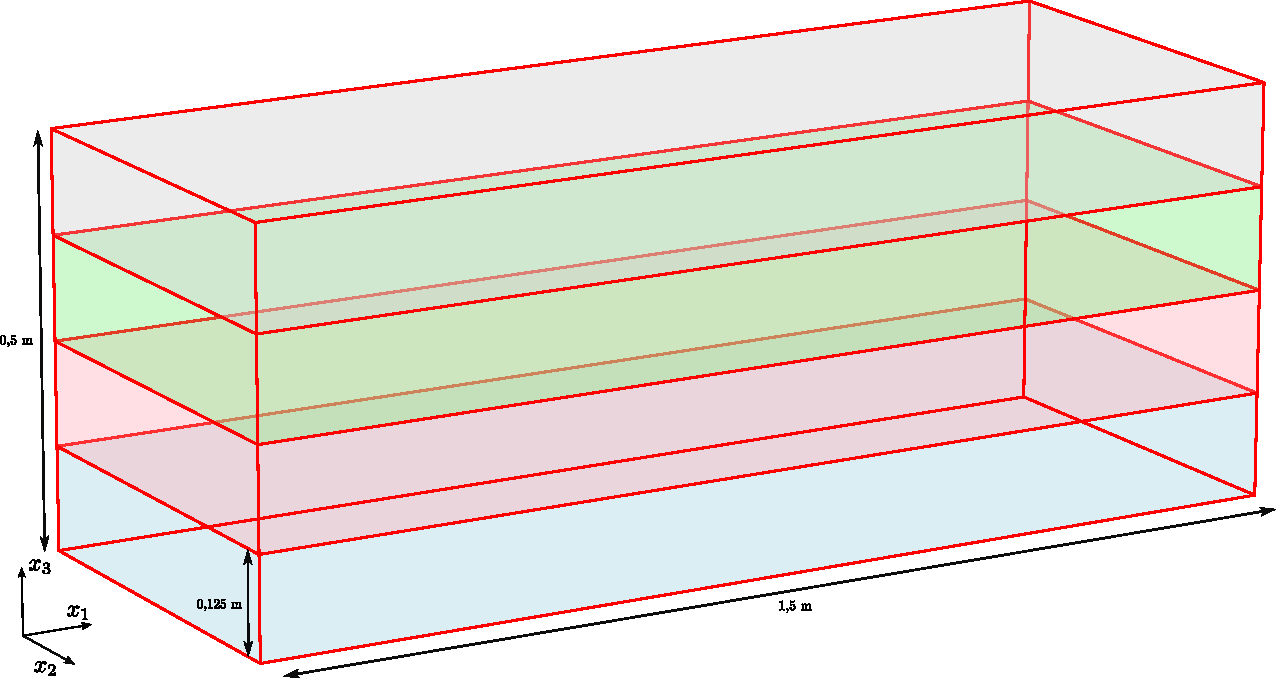
\includegraphics[width=.9\linewidth]{Img/Kapitola4/dif_dom.pdf}
            \caption{Sch\'{e}ma v\'{y}po\v{c}etn\'{\i} oblasti pro \'{u}lohu \ref{sub:Prob01}.}
            \label{fig:Probl01_domain}
        \end{figure}


        \begin{tcolorbox}[colframe=blue, title = \'{U}loha \ref{sub:Prob01}]
                            
            Parametry \'{u}lohy:
            \begin{itemize}
                \begin{multicols}{2}
                \item $\Omega = (0;1{,}0 \; \mathrm{m}) \times (0;0{,}5 \; \mathrm{m}) \times (0;0{,}5 \; \mathrm{m})$,
                \item $t \in \langle 0;0{,}1 \rangle \ \mathrm{s}$,
                \item $\nu = 1{,}552 \cdot 10^{-5} \ \mathrm{m^2 \ s^{-1}}$,
                \item $u_{in} = 2 \ \mathrm{m \ s^{-1}}$,
                \item $T_{ini} = 0 \ ^{\circ}\mathrm{C}$,
                \item $T_{in} = 25 \ ^{\circ}\mathrm{C}$,
                \item $D_{i} \in \{ 2{,}239 \cdot 10^{-i} \ | \ i \in \{ 1, 2, 3, 4\}\} \ \mathrm{m}^2 \ \mathrm{s}^{-1}$.
                \end{multicols}
            \end{itemize}
            
            Po\v{c}\'{a}te\v{c}n\'{\i} a okrajov\'{e} podm\'{\i}nky:
            \begin{itemize}
                \item V $\overline{\hat{\Omega}}$ nastav\'{\i}me po\v{c}\'{a}te\v{c}n\'{\i} podm\'{\i}nky dle sekc\'{\i} \ref{sec:NSEIniCon} a \ref{sec:ADEIniCon}.
                \item Na \v{c}\'{a}sti hranice $\hat{\Gamma}_{in}$ zvol\'{\i}me vstupn\'{\i} okrajov\'{e} podm\'{\i}nky popsan\'{e} v \ref{sec:NSEIniCon} a \ref{sec:ADEIniCon}.
                \item Pro $\hat{\Gamma}_{out}$ vol\'{\i}me odtokov\'{e} podm\'{\i}nky dle \ref{sec:NSEIniCon} a \ref{sec:ADEIniCon}.
                \item Na $\hat{\Gamma}_{w}$ pou\v{z}ijeme bounce-back okrajov\'{e} podm\'{\i}nky ze sekc\'{\i} \ref{sec:NSEIniCon} a \ref{sec:ADEIniCon}.
                \item Pro hranice mezi oblastmi p\v{r}edep\'{\i}\v{s}eme bounce-back okrajov\'{e} podm\'{\i}nky ze sekc\'{\i} \ref{sec:NSEIniCon} a \ref{sec:ADEIniCon}.
            \end{itemize}
            
            


            Parametry LBM:
            \begin{itemize}
                \item $N_x \times N_y \times N_z = (768 \times 384 \times 384)$,
                \item $\mathrm{Re} = 66 \ 666$,
                \item $\nu_{LBM} = 10^{-6}$, odpov\'{\i}d\'{a} $\Delta t \approx 10^{-7} s$.
            \end{itemize}

        \end{tcolorbox}

        \begin{figure}[H]
            \centering
            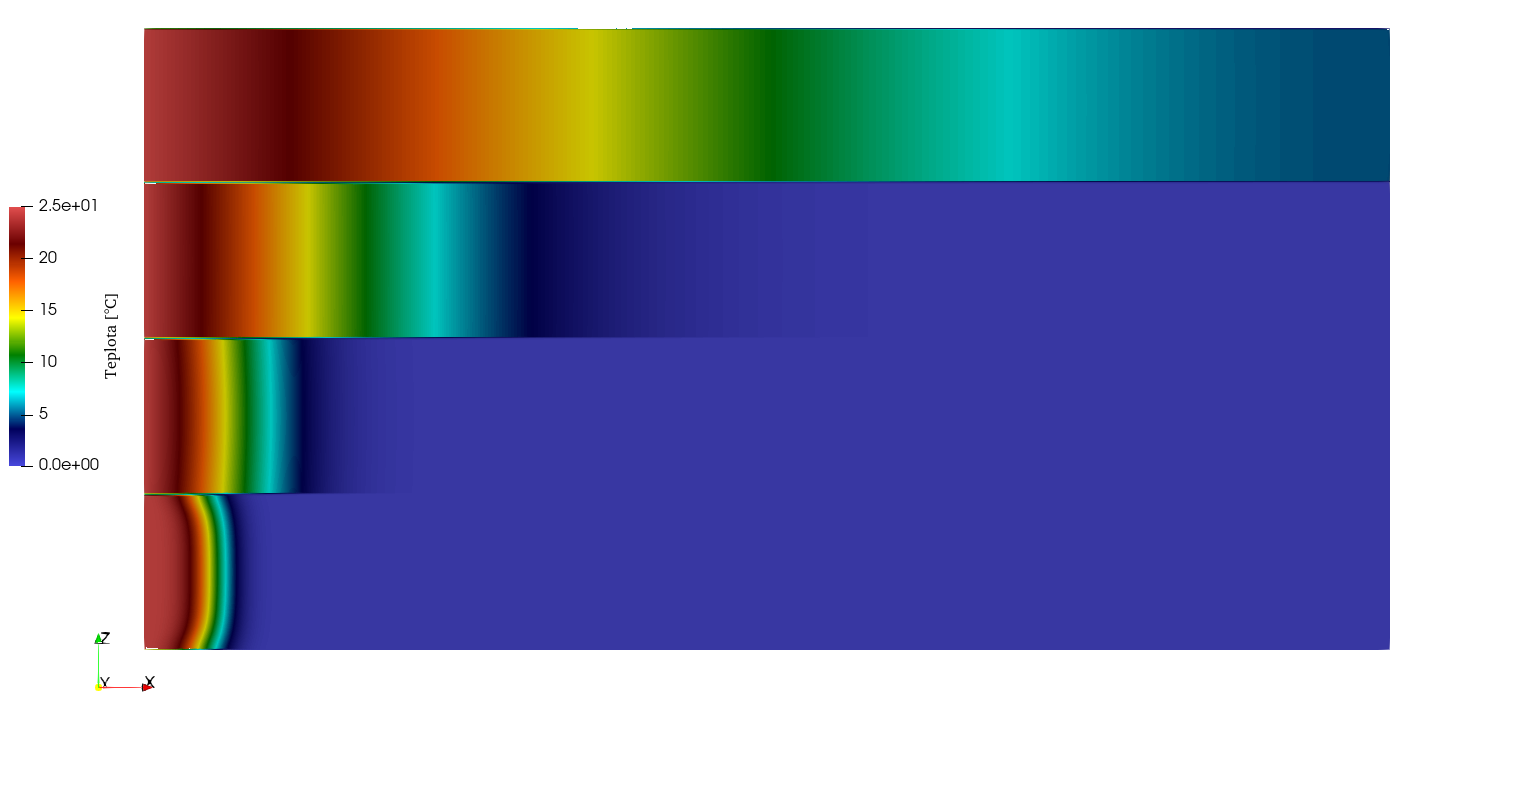
\includegraphics[width=\linewidth]{Img/Kapitola 3/Diffus_problem.png}
            \caption{Pr\r{u}\v{r}ez v\'{y}po\v{c}etn\'{\i} oblasti zn\'{a}zor\v{n}uj\'{\i}c\'{\i} \v{c}ty\v{r}i odd\v{e}len\'{e} \v{c}\'{a}sti oblasti s rozd\'{\i}ln\'{y}m difuzn\'{\i}m koeficientem $D_i$ pro $i \in \{1,2,3,4\}$ v \v{c}ase $t = 0{,}05 \ \mathrm{s}$. }
        \end{figure}
 


    \section{Testov\'{a}n\'{\i} p\v{r}estupov\'{e} okrajov\'{e} podm\'{\i}nky}
    \label{sec:TranConTest}

        V t\'{e}to sekci bude c\'{\i}lem otestovat implementovanou p\v{r}estupovovou okrajovou podm\'{\i}nku definovanou v sekci \ref{sec:TraBouCon}.
        
        Budeme uva\v{z}ovat 3D v\'{y}po\v{c}etn\'{\i} oblast ve tvaru kv\'{a}dru $\Omega = (0;1{,}5 \ \mathrm{m}) \times (0;0{,}5 \ \mathrm{m}) \times (0;0{,}5 \ \mathrm{m})$. Do n\'{\i} bude pevn\v{e} um\'{\i}st\v{e}no kv\'{a}drov\'{e} t\v{e}leso $\Omega_b$ o rozm\v{e}rech $(0{,}0252 \ \mathrm{m} \times 0{,}245 \ \mathrm{m} \times 0{,}105 \ \mathrm{m})$ s po\v{c}\'{a}te\v{c}n\'{\i} teplotou $T_{ini,b}$, viz obr\'{a}zek \ref{fig:Probl02_domain}. 
        
        P\v{r}i simulac\'{i}ch budeme uva\v{z}ovat r\r{u}zn\'{e} hodnoty jak pro koeficient p\v{r}estupu $\omega$, tak i pro velikost vstupn\'{\i} rychlosti $u_{in}$. D\'{a}le uva\v{z}ujeme i r\r{u}zn\'{e} prostorov\'{e} kroky $h$. P\v{r}edm\v{e}tem z\'{a}jmu pro n\'{a}s bude pr\r{u}m\v{e}rn\'{a} teplota na t\v{e}lese $\Omega_b$.

        \begin{figure}[H]
            \centering
            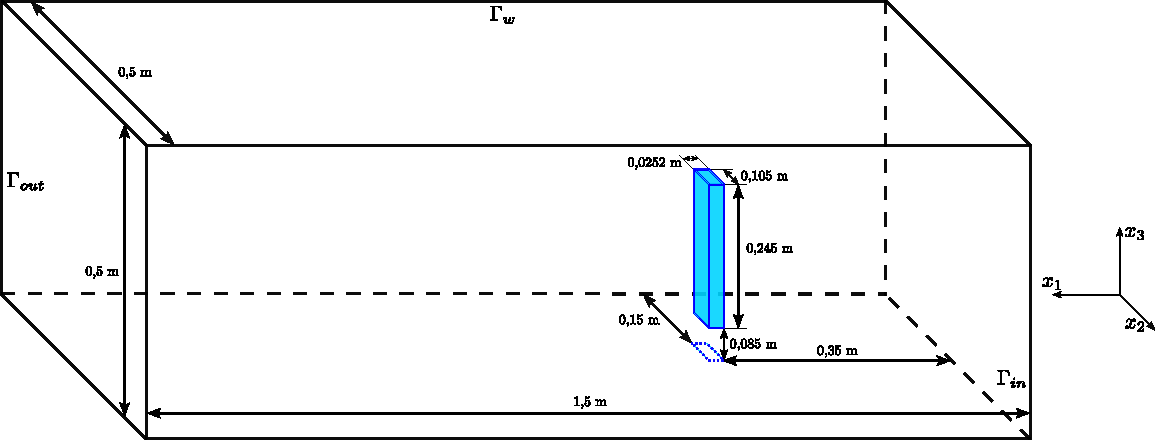
\includegraphics[width=\linewidth]{Img/Kapitola 3/Radiator_domain_without_mono.pdf}
            \caption{Sch\'{e}ma v\'{y}po\v{c}etn\'{\i} oblasti pro \'{u}lohu \ref{sub:Prob02}.}
            \label{fig:Probl02_domain}
        \end{figure}

        % C\'{\i}lem t\'{e}to sekce je ov\v{e}\v{r}it spr\'{a}vnost implementace v\'{y}po\v{c}tu s\'{\i}ly metodou v\'{y}m\v{e}ny hybnosti popsan\'{e} v sekci \ref{sec:MomExcMet}. Jeden z p\v{r}\'{\i}stup\r{u}, jak zjistit spr\'{a}vnost na\v{s}eho modelu, je pomoc\'{\i} bezrozm\v{e}rn\'{y}ch veli\v{c}in. V~na\v{s}em p\v{r}\'{\i}pad\v{e} se zam\v{e}\v{r}\'{\i}me na odporov\'{y} a vztlakov\'{y} koeficient.
        
        
        % Implementaci v\'{y}po\v{c}tu s\'{\i}ly ov\v{e}\v{r}\'{\i}me v\'{y}po\v{c}tem odporov\'{e}ho a vztlakov\'{e}ho koeficientu pomoc\'{\i} vztah\r{u} \eqref{eq:DraCoe} a \eqref{eq:LifCoe} aplikovan\'{y}ch na v\'{a}lec o polom\v{e}ru $r = 0{,}05 \ \mathrm{m}$, tj.
        
        % \begin{subequations}
        % \label{eq:NumCoe}
        % \begin{align}
        %     c_D = \frac{2F_1}{\rho U^{2}_{\infty}S}, \label{eq:NumDraCoe} \\
        %     c_L = \frac{2F_2}{\rho {U}^{2}_{\infty}S}, \label{eq:NumLifCoe}
        % \end{align}
        % \end{subequations}
        % kde $F_1,F_2$ jsou slo\v{z}ky vektoru s\'{\i}ly a $S = 0{,}1 \ \mathrm{m^2}$ odpov\'{\i}d\'{a} obsahu podstavy t\v{e}lesa dle \cite{schafer1996benchmark}. Na vstupu budeme p\v{r}edepisovat podm\'{\i}nky $P$ a $G$ definovan\'{e} v sekci \ref{sub:InfCon} a rychlost s parabolick\'{y}m profilem danou vztahem \eqref{eq:DefCasConInl2}. Dle maxim\'{a}ln\'{\i} p\v{r}edepisovan\'{e} rychlosti rozd\v{e}l\'{\i}me tuto \'{u}lohu na dv\v{e} pod\'{u}lohy: stabiln\'{\i} (s $U_{\infty} = 0{,}3 \ \mathrm{ m \; s^{-1}}$) a nestabiln\'{\i} (s $U_{\infty} = 1{,}5 \ \mathrm{ m \; s^{-1}}$).
        
        % \begin{figure}[H]
        %     \centering
        %     \includegraphics{Img/Kapitola 3/STurek3-1.pdf}
        %     \caption{Sch\'{e}ma um\'{\i}st\v{e}n\'{\i} kruhov\'{e}ho t\v{e}lesa o polom\v{e}ru podstavy $r = 0{,}05 \ \mathrm{m}$ ve 2D v\'{y}po\v{c}etn\'{\i} oblasti $\Omega = (0;1{,}64 \; \mathrm{m}) \times (0;0{,}41 \; \mathrm{m})$.}
        %     \label{fig:DomainST}
        % \end{figure}
        
        \subsection{P\v{r}estupov\'{a} OP}
        \label{sub:Prob02}
        
    
        \begin{tcolorbox}[colframe=blue, title = \'{U}loha \ref{sub:Prob02}]
                            
            Parametry \'{u}lohy:
            \begin{itemize}
                \begin{multicols}{2}
                \item $\Omega = (0;1{,}5 \; \mathrm{m}) \times (0;0{,}5 \; \mathrm{m}) \times (0;0{,}5 \; \mathrm{m})$,
                \item $t \in \langle 0;0{,}1 \rangle \ \mathrm{s}$,
                \item $\nu = 1{,}552 \cdot 10^{-5} \ \mathrm{m^2 \ s^{-1}}$,
                \item $u_{in} \in \{ 1, 4, 8, 12, 16, 20 \} \ \mathrm{m \ s^{-1}}$, 
                \item $T_{ini,a} = 25 \ ^{\circ}\mathrm{C}$,
                \item $T_{in} = 25 \ ^{\circ}\mathrm{C}$,
                \item $T_{ini,b} = 75 \ ^{\circ}\mathrm{C}$,
                \item $D_{a} = 2{,}239 \cdot 10^{-5} \ \mathrm{m^2 \ s^{-1}}$, 
                \item $D_b = 9{,}700 \cdot 10^{-5} \ \mathrm{m^2 \ s^{-1}}$,
                \item $\omega = 0{,}05j$ \quad $\forall j \in \{ 1,2,\dots,20 \} \ \mathrm{kg \ s^{-3} \ K^{-1}}$.
                \end{multicols}
            \end{itemize}
            
            Po\v{c}\'{a}te\v{c}n\'{\i} a okrajov\'{e} podm\'{\i}nky:
            \begin{itemize}
                \item V $\overline{\hat{\Omega}}$ nastav\'{\i}me po\v{c}\'{a}te\v{c}n\'{\i} podm\'{\i}nky dle sekc\'{\i} \ref{sec:NSEIniCon} a \ref{sec:ADEIniCon}.
                \item Na \v{c}\'{a}sti hranice $\hat{\Gamma}_{in}$ zvol\'{\i}me vstupn\'{\i} okrajov\'{e} podm\'{\i}nky popsan\'{e} v \ref{sec:NSEIniCon} a \ref{sec:ADEIniCon}.
                \item Pro $\hat{\Gamma}_{out}$ vol\'{\i}me odtokov\'{e} podm\'{\i}nky dle \ref{sec:NSEIniCon} a \ref{sec:ADEIniCon}.
                \item Na $\hat{\Gamma}_{w}$ pou\v{z}ijeme bounce-back okrajov\'{e} podm\'{\i}nky ze sekc\'{\i} \ref{sec:NSEIniCon} a \ref{sec:ADEIniCon}.
                \item Pro t\v{e}leso $\overline{\hat{\Omega}}_b$ vol\'{\i}me n\'{a}sleduj\'{\i}c\'{\i} okrajov\'{e} podm\'{\i}nky: \begin{itemize}
                    \item Pro NSR sch\'{e}ma vol\'{\i}me na $\overline{\hat{\Omega}}_b$ bounce-back okrajovou podm\'{\i}nku dle \ref{sec:NSEIniCon},
                    \item V ADR sch\'{e}matu pou\v{z}ijeme na $\hat{\Gamma}_b$ p\v{r}estupovou podm\'{\i}nku, viz \ref{sec:ADEIniCon}.  
                \end{itemize}
            \end{itemize}
            
            Parametry LBM:
            \begin{itemize}
                \item $N_x \times N_y \times N_z \in \{ 96i \times 32i \times 32i\ | \ i \in \{ 3,4,\dots,8 \} \} $,
                \item $\mathrm{Re} \in \langle 33 \ 333, 666 \ 666 \rangle$,
                \item $\nu_{LBM} = 10^{-6}$, odpov\'{\i}d\'{a} $\Delta t \approx 10^{-7} s$.
            \end{itemize}

        \end{tcolorbox}
        
        
        \begin{figure}[H]
            \centering
            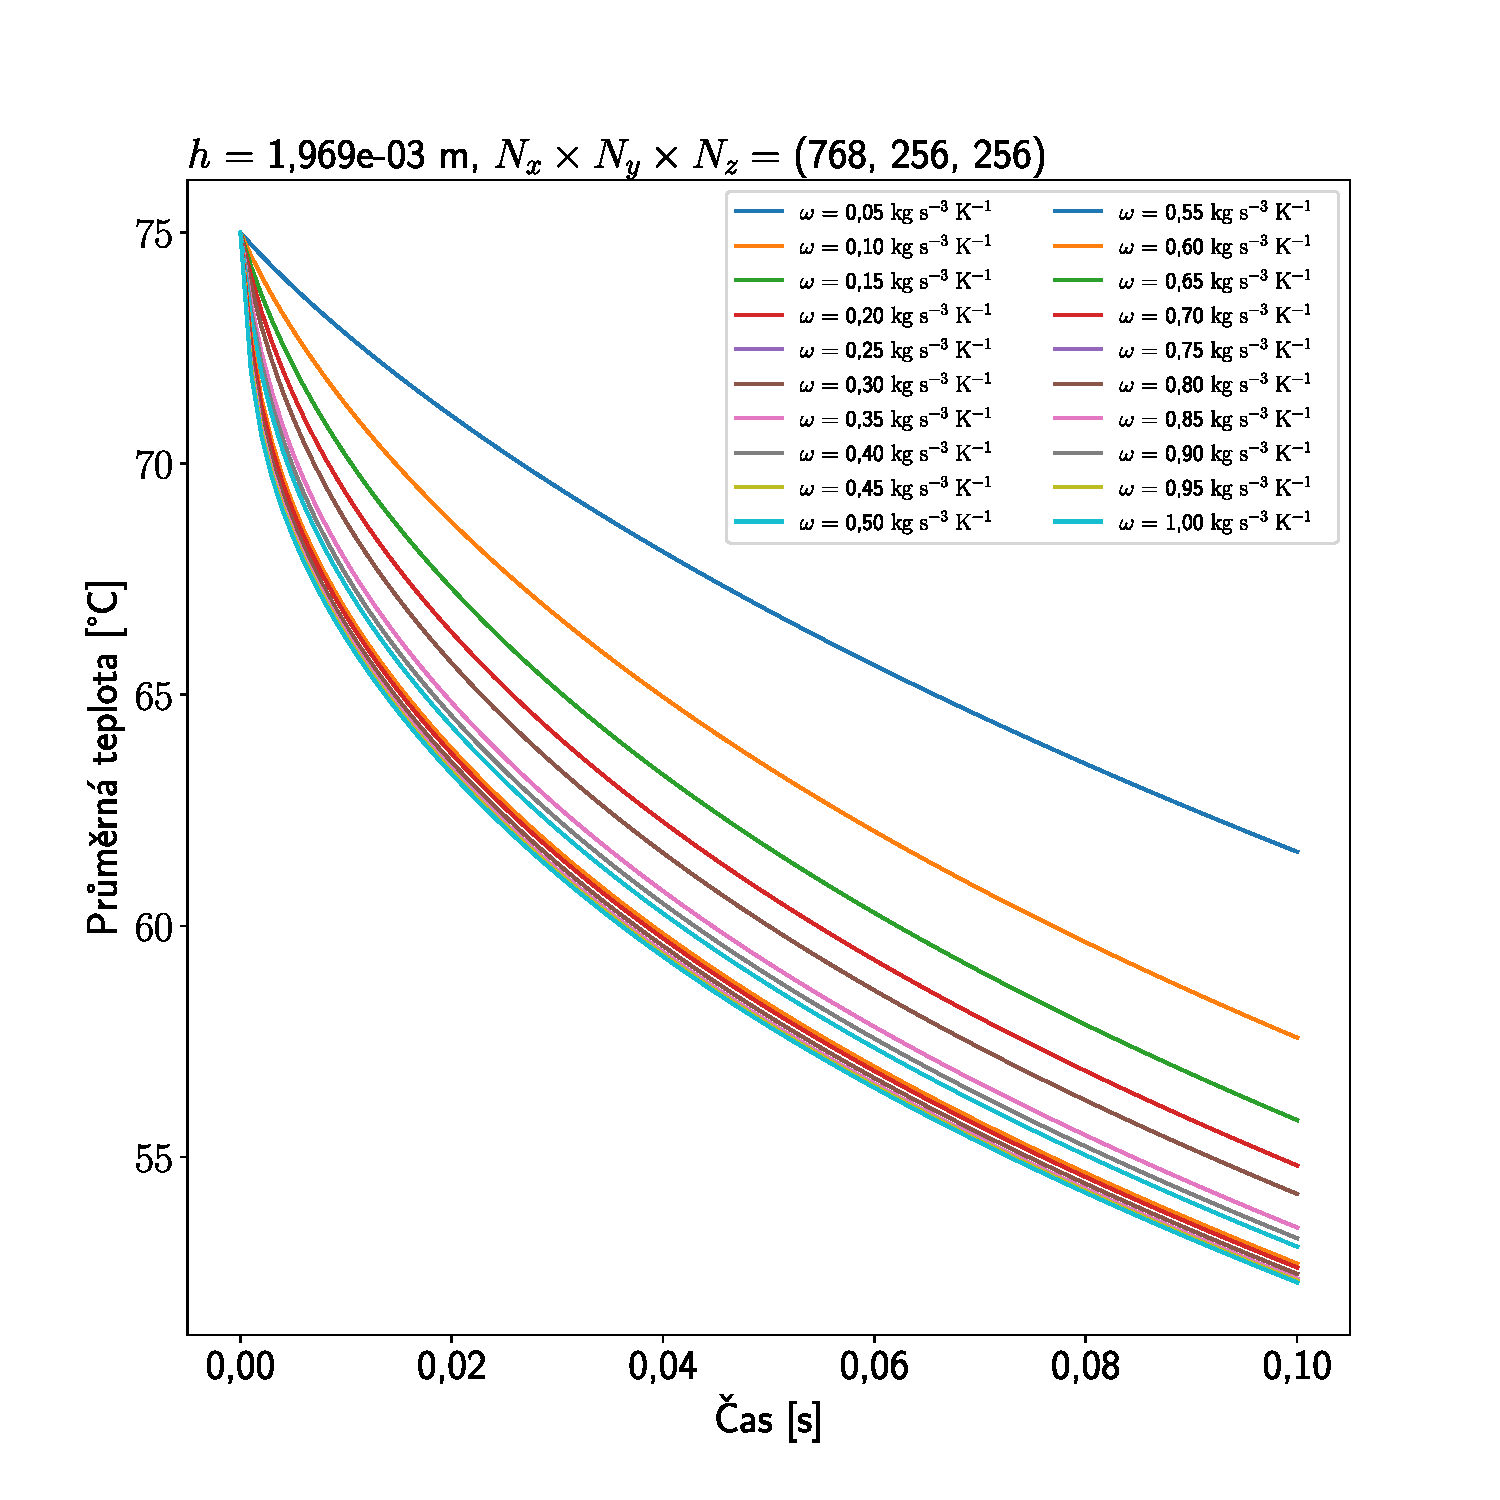
\includegraphics[width=.95\linewidth, clip, trim=1.45cm 0.95cm 2cm 1.7cm]{Img/Kapitola 3/Problem02_all_transfers.pdf}
            \caption{Graf z\'{a}vislosti pr\r{u}m\v{e}rn\'{e} teploty na t\v{e}lese $\Omega_b$ na \v{c}ase $t$ pro \'{u}lohu \ref{sub:Prob02} a pro r\r{u}zn\'{e} hodnoty koeficientu p\v{r}estupu $\omega$, prostorov\'{y} krok $h = 1{,}969\cdot 10^{-3} \ \mathrm{m}$ odpov\'{\i}daj\'{\i}c\'{\i} m\v{r}\'{\i}\v{z}ce (768, 256, 256), \v{c}asov\'{y} krok $\Delta t =  2{,}497 \cdot 10^{-7}$ s a velikost vstupn\'{\i} rychlosti $u_{in} = 1 \ \mathrm{m \ s^{-1}}$. }
            \label{fig:Prob05_diff_h}
        \end{figure}

        \begin{figure}[H]
            \centering
            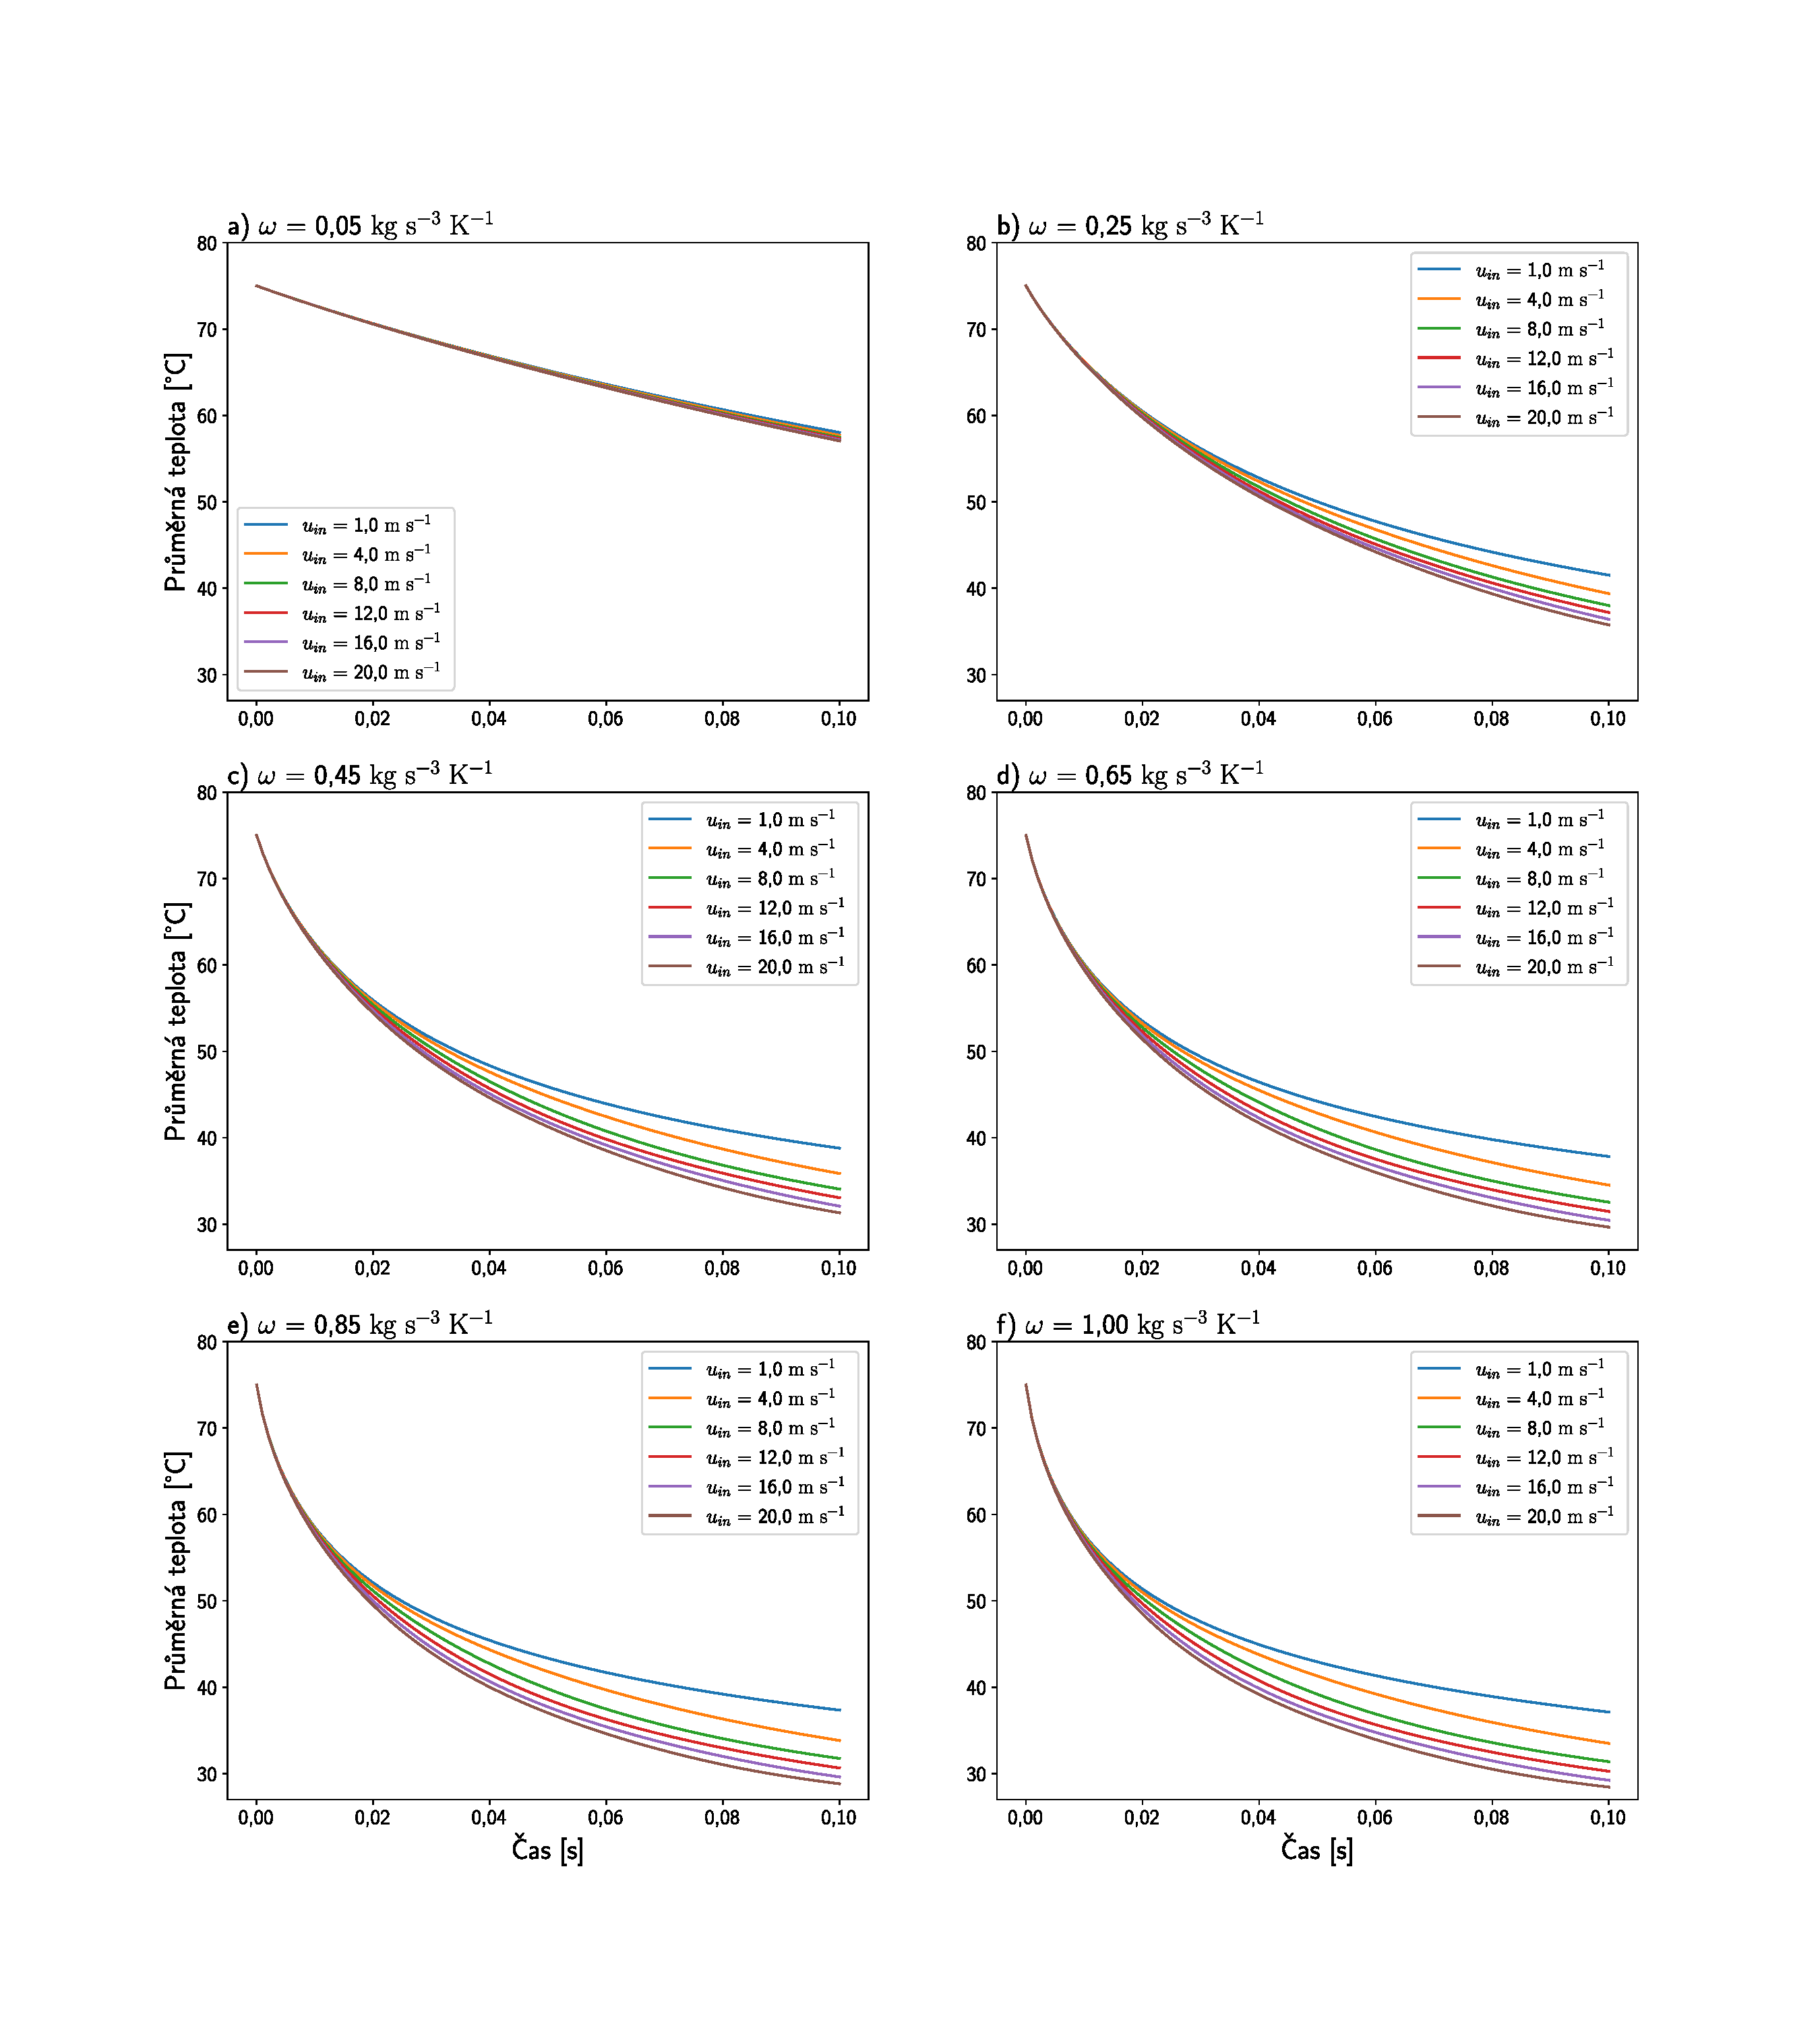
\includegraphics[width=\linewidth, trim=4cm 4cm 4cm 8cm]{Img/Kapitola 3/Probl10_a.pdf}
            \caption{Grafy zobrazuj\'{\i}c\'{\i} z\'{a}vislost pr\r{u}m\v{e}rn\'{e} teploty $T$ na \v{c}ase $t$ pro \'{u}lohu \ref{sub:Prob02} a pro r\r{u}zn\'{e} velikosti vstupn\'{\i} rychlosti $u_{in}$. Vyobrazeny jsou grafy pro r\r{u}zn\'{e} volby koeficientu p\v{r}estupu $\omega$. Ve v\v{s}ech grafech uva\v{z}ujeme prostorov\'{y} krok $h = 1{,}969 \cdot 10^{-3} \ \mathrm{m}$ odpov\'{\i}daj\'{\i}c\'{\i} m\v{r}\'{\i}\v{z}ce (768, 256, 256) a \v{c}asov\'{y} krok $\Delta t = 1{,}015 \cdot 10^{-7} \ \mathrm{s}$.}
            \label{fig:Probl10_a}
        \end{figure}

        \begin{figure}[H]
            \centering
            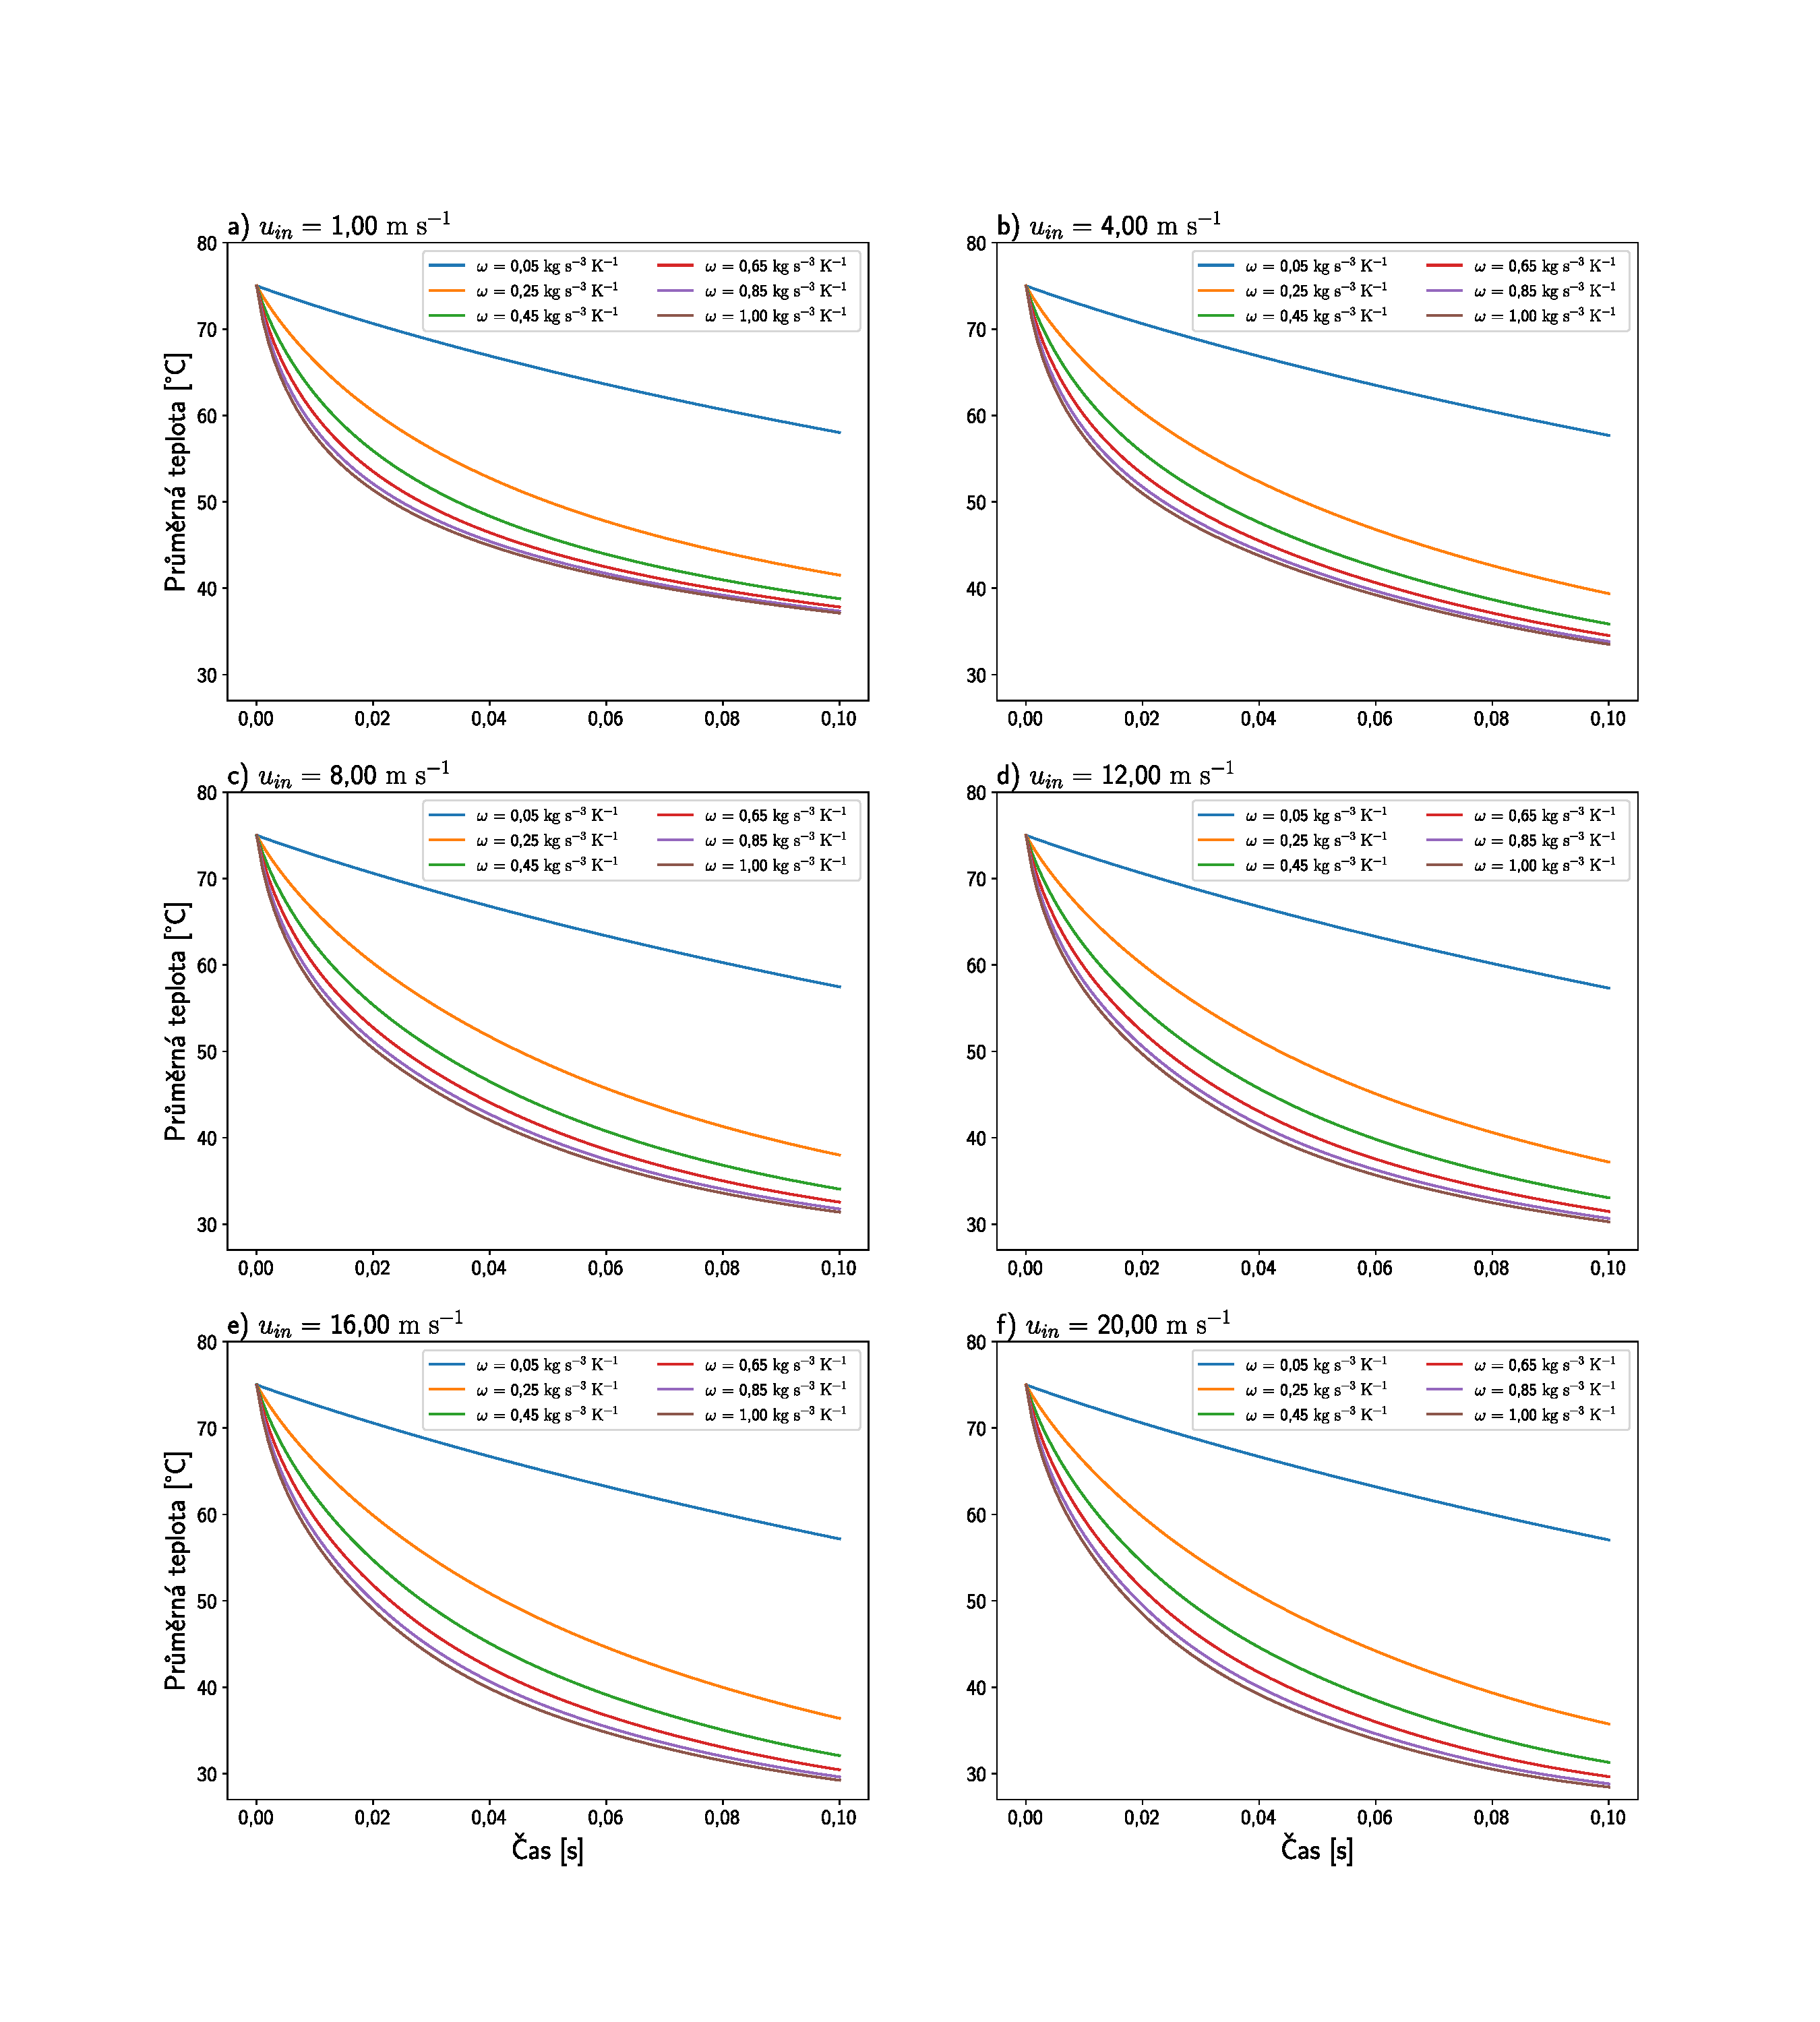
\includegraphics[width=\linewidth, trim=4cm 4cm 4cm 8cm]{Img/Kapitola 3/Probl10_b.pdf}
            \caption{Grafy zobrazuj\'{\i}c\'{\i} z\'{a}vislost pr\r{u}m\v{e}rn\'{e} teploty $T$ na \v{c}ase $t$ pro \'{u}lohu \ref{sub:Prob02} a pro r\r{u}zn\'{e} hodnoty koeficientu p\v{r}estupu $\omega$. Vyobrazeny jsou grafy pro r\r{u}zn\'{e} hodnoty vstupn\'{\i} rychlosti $u_{in}$. Ve v\v{s}ech grafech uva\v{z}ujeme prostorov\'{y} krok $h = 1{,}969 \cdot 10^{-3} \ \mathrm{m}$ odpov\'{\i}daj\'{\i}c\'{\i} m\v{r}\'{\i}\v{z}ce (768, 256, 256) a \v{c}asov\'{y} krok $\Delta t = 1{,}015 \cdot 10^{-7} \ \mathrm{s}$.}
            \label{fig:Probl10_b}
        \end{figure}





        \subsection{V\'{y}sledky \'{u}lohy \ref{sub:Prob02}}

            \'{U}loha \ref{sub:Prob02} simuluje nastaven\'{\i} p\v{r}estupov\'{e} okrajov\'{e} podm\'{\i}nky v modelu. P\v{r}edm\v{e}tem zkoum\'{a}n\'{\i} zde je v\'{y}voj pr\r{u}m\v{e}rn\'{e} teploty $T_{mean}$ v \v{c}ase $t$. Na grafu \ref{fig:Prob05_diff_h} pozorujeme z\'{a}vislost pr\r{u}m\v{e}rn\'{e} teploty pro r\r{u}zn\'{e} koeficienty p\v{r}estupu $\omega$ a vstupn\'{\i} rychlost $u_{in} = 1 \ \mathrm{m \ s^{-1}}$. Z grafu je z\v{r}ejm\'{e}, \v{z}e se zvy\v{s}uj\'{\i}c\'{\i} se hodnotou $\omega$ se \'{u}\v{c}innost chlazen\'{\i} zvy\v{s}uje a\v{z} do ur\v{c}it\'{e}ho limitn\'{\i}ho stavu. Na obr\'{a}zku \ref{fig:Probl10_b} je tato situace vyobrazena pro r\r{u}zn\'{e} hodnoty po\v{c}\'{a}te\v{c}n\'{\i} rychlosti $u_{in}$ a pro vybran\'{e} koeficienty p\v{r}estupu $\omega$. Lze nahl\'{e}dnout, \v{z}e i pro vy\v{s}\v{s}\'{\i} hodnoty vstupn\'{\i} rychlosti pr\r{u}m\v{e}rn\'{e} teploty konverguj\'{\i}.
        
            Z obr\'{a}zku \ref{fig:Probl10_a} lze vy\v{c}\'{\i}st, \v{z}e pro mal\'{e} koeficienty p\v{r}estupu t\'{e}m\v{e}\v{r} nez\'{a}vis\'{\i} na velikosti vstupn\'{\i} rychlosti. Pro hodnoty $\omega$ bl\'{\i}zk\'{e} 1 jsou ji\v{z} rozd\'{\i}ly mezi pr\r{u}m\v{e}rn\'{y}mi teplotami nezanedbateln\'{e}, ale i p\v{r}esto tyto rozd\'{\i}ly nejsou tak markantn\'{\i} v porovn\'{a}n\'{\i} s rychlostmi na vstupu. 
        

        \subsection{Pozn\'{a}mka k implementaci p\v{r}estupov\'{e} okrajov\'{e} podm\'{\i}nky}

            P\v{r}i implementaci p\v{r}estupov\'{e} okrajov\'{e} podm\'{\i}nky do\v{s}lo k odhalen\'{\i} chyby, kv\r{u}li kter\'{e} teplota unikala do okol\'{\i} i p\v{r}i nulov\'{e}m koeficientu p\v{r}estupu. Po lokalizaci chyby bylo zji\v{s}teno, \v{z}e probl\'{e}m nast\'{a}v\'{a} v situaci, kdy dojde ke kontaktu st\v{e}n oblasti s p\v{r}ek\'{a}\v{z}kou, tj. $\exists k \in \{0,1,2,\dots,6\}$ takov\'{e}, \v{z}e
            \begin{equation}
                g(\boldsymbol{x}_b + \xi_k \Delta t, t) = g(\boldsymbol{x}_w, t), 
            \end{equation}
            pro n\v{e}jak\'{e} uzly $\boldsymbol{x}_b$ a $\boldsymbol{x}_w$ ozna\v{c}uj\'{\i}c\'{\i} po \v{r}ad\v{e} uzel t\v{e}lesa a uzel st\v{e}ny. 
        
            Pro vy\v{r}e\v{s}en\'{\i} t\'{e}to chyby se nakonec uk\'{a}zalo nutn\'{e} do p\v{r}estupov\'{e} podm\'{\i}nky zahrnout je\v{s}t\v{e} i tento p\v{r}\'{\i}pad, tedy situaci, kdy se uzly t\v{e}lesa nach\'{a}z\'{\i} v kontaktu s uzlem zdi.


        

    % \section{Hled\'{a}n\'{\i} optim\'{a}ln\'{\i}ho rozm\v{e}ru radi\'{a}toru}
    % \label{sec:OptRad}
    
    %     Tato sekce se bude v\v{e}novat hled\'{a}n\'{\i} optim\'{a}ln\'{\i}ho tvaru radi\'{a}toru pro v\r{u}z studentsk\'{e} elektrick\'{e} formule FSE.12. Jak ji\v{z} bylo zm\'{\i}n\v{e}no, chlad\'{\i}c\'{\i} syst\'{e}m se nach\'{a}z\'{\i} v zadn\'{\i} \v{c}\'{a}sti vozu, proto p\v{r}i modelov\'{a}n\'{\i} v\'{y}po\v{c}etn\'{\i} oblasti lze \v{c}\'{a}ste\v{c}n\v{e} zanedbat geometrii p\v{r}edn\'{\i} \v{c}\'{a}sti vozu.

    %     Budeme uva\v{z}ovat op\v{e}t 3D v\'{y}po\v{c}etn\'{\i} oblast ve tvaru kv\'{a}dru $\Omega = (0;1{,}5 \ \mathrm{m}) \times (0;0{,}5 \ \mathrm{m}) \times (0;0{,}5 \ \mathrm{m})$, do kter\'{e} budou vlo\v{z}eny 2 t\v{e}lesa. Prvn\'{\i} z nich p\v{r}edstavuje \v{c}\'{a}st monokoku formule $\Omega_m$, kter\'{y} je um\'{\i}st\v{e}n jako na obr\'{a}zku \ref{fig:Probl06_domain}. Toto t\v{e}leso se bude v p\v{r}\'{\i}pad\v{e} \v{r}e\v{s}en\'{\i} NSR i ADR chovat jako pevn\'{a} p\v{r}ek\'{a}\v{z}ka, od kter\'{e} se vzduch i teplota odr\'{a}\v{z}\'{\i}. Druh\'{e} t\v{e}leso $\Omega_r$ p\v{r}edstavuje primitivn\'{\i} chladi\v{c}, u kter\'{e}ho prozat\'{\i}m zanedb\'{a}v\'{a}me geometrii vo\v{s}tiny, tud\'{\i}\v{z} v modelu je vyobrazen jako kv\'{a}dr. Chladi\v{c} se bude pro sch\'{e}ma NSR chovat jako pevn\'{a} p\v{r}ek\'{a}\v{z}ka, p\v{r}i \v{r}e\v{s}en\'{\i} ADR sch\'{e}matu budeme uva\v{z}ovat po\v{c}\'{a}te\v{c}n\'{\i} teplotu chladi\v{c}e $T_{ini,b}$. P\v{r}edpokl\'{a}dejme, \v{z}e radi\'{a}tor je vyroben z hlin\'{\i}ku. 
        
    %     % Po\v{z}adovan\'{a} plocha chladi\v{c}e kolm\'{a} na osu $x$ byla stanovena na $S\approx 25 000 \ \mathrm{mm^2}$. Navrhnut\'{e} a testovan\'{e} rozm\v{e}ry chladi\v{c}e byly zvoleny dle platn\'{y}ch pravidel a mo\v{z}nost\'{\i} v\'{y}robce.

    %     C\'{\i}lem t\'{e}to \'{u}lohy bude porovnat v\'{y}sledky pr\r{u}m\v{e}n\'{y}ch teplot $T_{mean}$ na chladi\v{c}\'{\i}ch a tak rozhodnout, jak\'{e} rozm\v{e}ry chladi\v{c}e jsou optim\'{a}ln\'{\i} pro takto zvolenou \'{u}lohu.
            
    %     \begin{figure}[H]
    %         \centering
    %         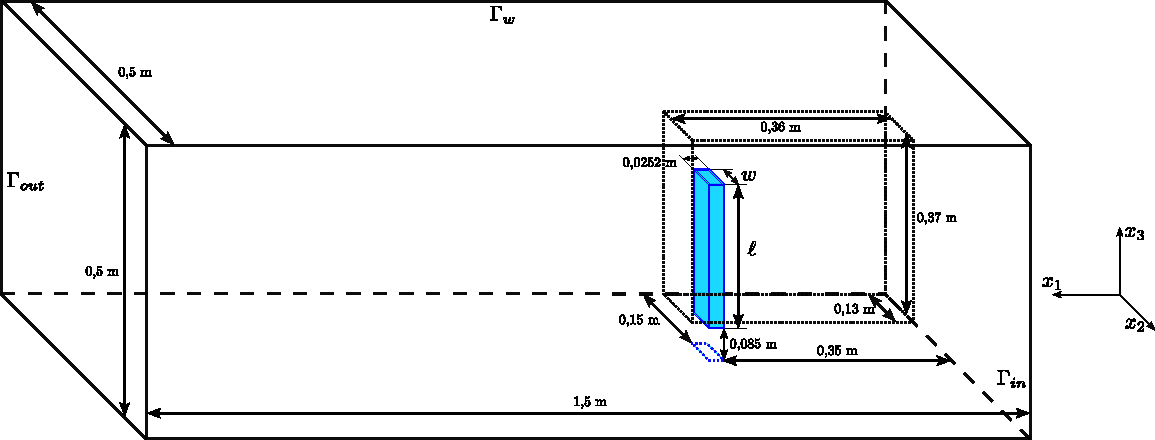
\includegraphics[width=\linewidth]{Img/Kapitola 3/Radiator_domain_with_mono.pdf}
    %         \caption{Sch\'{e}ma v\'{y}po\v{c}etn\'{\i} oblasti pro \'{u}lohu \ref{sub:Prob06}, kde \v{s}\'{\i}\v{r}ka $w$ a v\'{y}\v{s}ka $\ell$ v\'{y}m\v{e}n\'{\i}ku jsou parametry \'{u}lohy.}
    %         \label{fig:Probl06_domain}
    %     \end{figure}
        

    %     \subsection{Hled\'{a}n\'{\i} optim\'{a}ln\'{\i}ho chladi\v{c}e}
    %     \label{sub:Prob06}
        
    %         \begin{tcolorbox}[colframe=blue, title = \'{U}loha \ref{sub:Prob06}]
                                
    %             Parametry \'{u}lohy:
    %             \begin{itemize}
    %                 \begin{multicols}{2}
    %                 \item $\Omega = (0;1{,}5 \; \mathrm{m}) \times (0;0{,}5 \; \mathrm{m}) \times (0;0{,}5 \; \mathrm{m})$,
    %                 \item $t \in \langle 0;0{,}1 \rangle \ \mathrm{s}$,
    %                 \item $\nu = 1{,}552 \cdot 10^{-5} \ \mathrm{m^2 \ s^{-1}}$,
    %                 \item $u_{in} = 16 \ \mathrm{m \ s^{-1}}$, 
    %                 \item $T_{ini,a} = 25 \ ^{\circ}\mathrm{C}$,
    %                 \item $T_{in} = 25 \ ^{\circ}\mathrm{C}$,
    %                 \item $T_{ini,b} = 75 \ ^{\circ}\mathrm{C}$,
    %                 \item $D_{a} = 2{,}239 \cdot 10^{-5} \ \mathrm{m^2 \ s^{-1}}$, 
    %                 \item $D_b = 9{,}700 \cdot 10^{-5} \ \mathrm{m^2 \ s^{-1}}$,
    %                 \item $\omega = 1 \ \mathrm{kg \ s^{-3} \ K^{-1}}$.
    %                 \end{multicols}
    %                 \item ($w$,$\ell$) $\in \{ (250;100), (245;100), (245;105), (240;105), (235,105), (235,110), (230,110), \\ (225,110), (225,115), (220,110), (220,115), (215,115), (215,120), (210, 120), (210,115), \\ (205,120), (205,125), (200,125), (200,120), (200,130), (195,125), (195,130), (190,130), \\(190,135), (185,135) \} \ \mathrm{mm}$ 
    %             \end{itemize}
                
    %             Po\v{c}\'{a}te\v{c}n\'{\i} a okrajov\'{e} podm\'{\i}nky:
    %             \begin{itemize}
    %                 \item V $\overline{\hat{\Omega}}$ nastav\'{\i}me po\v{c}\'{a}te\v{c}n\'{\i} podm\'{\i}nky dle sekc\'{\i} \ref{sec:NSEIniCon} a \ref{sec:ADEIniCon}.
    %                 \item Na \v{c}\'{a}sti hranice $\hat{\Gamma}_{in}$ zvol\'{\i}me vstupn\'{\i} okrajov\'{e} podm\'{\i}nky popsan\'{e} v \ref{sec:NSEIniCon} a \ref{sec:ADEIniCon}.
    %                 \item Pro $\hat{\Gamma}_{out}$ vol\'{\i}me odtokov\'{e} podm\'{\i}nky dle \ref{sec:NSEIniCon} a \ref{sec:ADEIniCon}.
    %                 \item Na $\hat{\Gamma}_{w}$ pou\v{z}ijeme bounce-back okrajov\'{e} podm\'{\i}nky ze sekc\'{\i} \ref{sec:NSEIniCon} a \ref{sec:ADEIniCon}.
    %                 \item Pro t\v{e}leso $\overline{\hat{\Omega}}_b$ vol\'{\i}me n\'{a}sleduj\'{\i}c\'{\i} okrajov\'{e} podm\'{\i}nky: \begin{itemize}
    %                     \item Pro NSR sch\'{e}ma vol\'{\i}me na $\overline{\hat{\Omega}}_b$ bounce-back okrajovou podm\'{\i}nku dle \ref{sec:NSEIniCon},
    %                     \item V ADR sch\'{e}matu pou\v{z}ijeme na $\hat{\Gamma}_b$ p\v{r}estupovou podm\'{\i}nku, viz \ref{sec:ADEIniCon}.  
    %                 \end{itemize}
    %             \end{itemize}
                
    %             Parametry LBM:
    %             \begin{itemize}
    %                 \item $N_x \times N_y \times N_z \in \{ 96i \times 32i \times 32i\ | \ i \in \{ 3,4,\dots,8 \} \} $,
    %                 \item $\mathrm{Re} \approx 533 \ 333$,
    %                 \item $\nu_{LBM} = 10^{-6}$, odpov\'{\i}d\'{a} $\Delta t \approx 10^{-7} s$.
    %             \end{itemize}

    %         \end{tcolorbox}

    %         \begin{figure}[H]
    %             \centering
    %             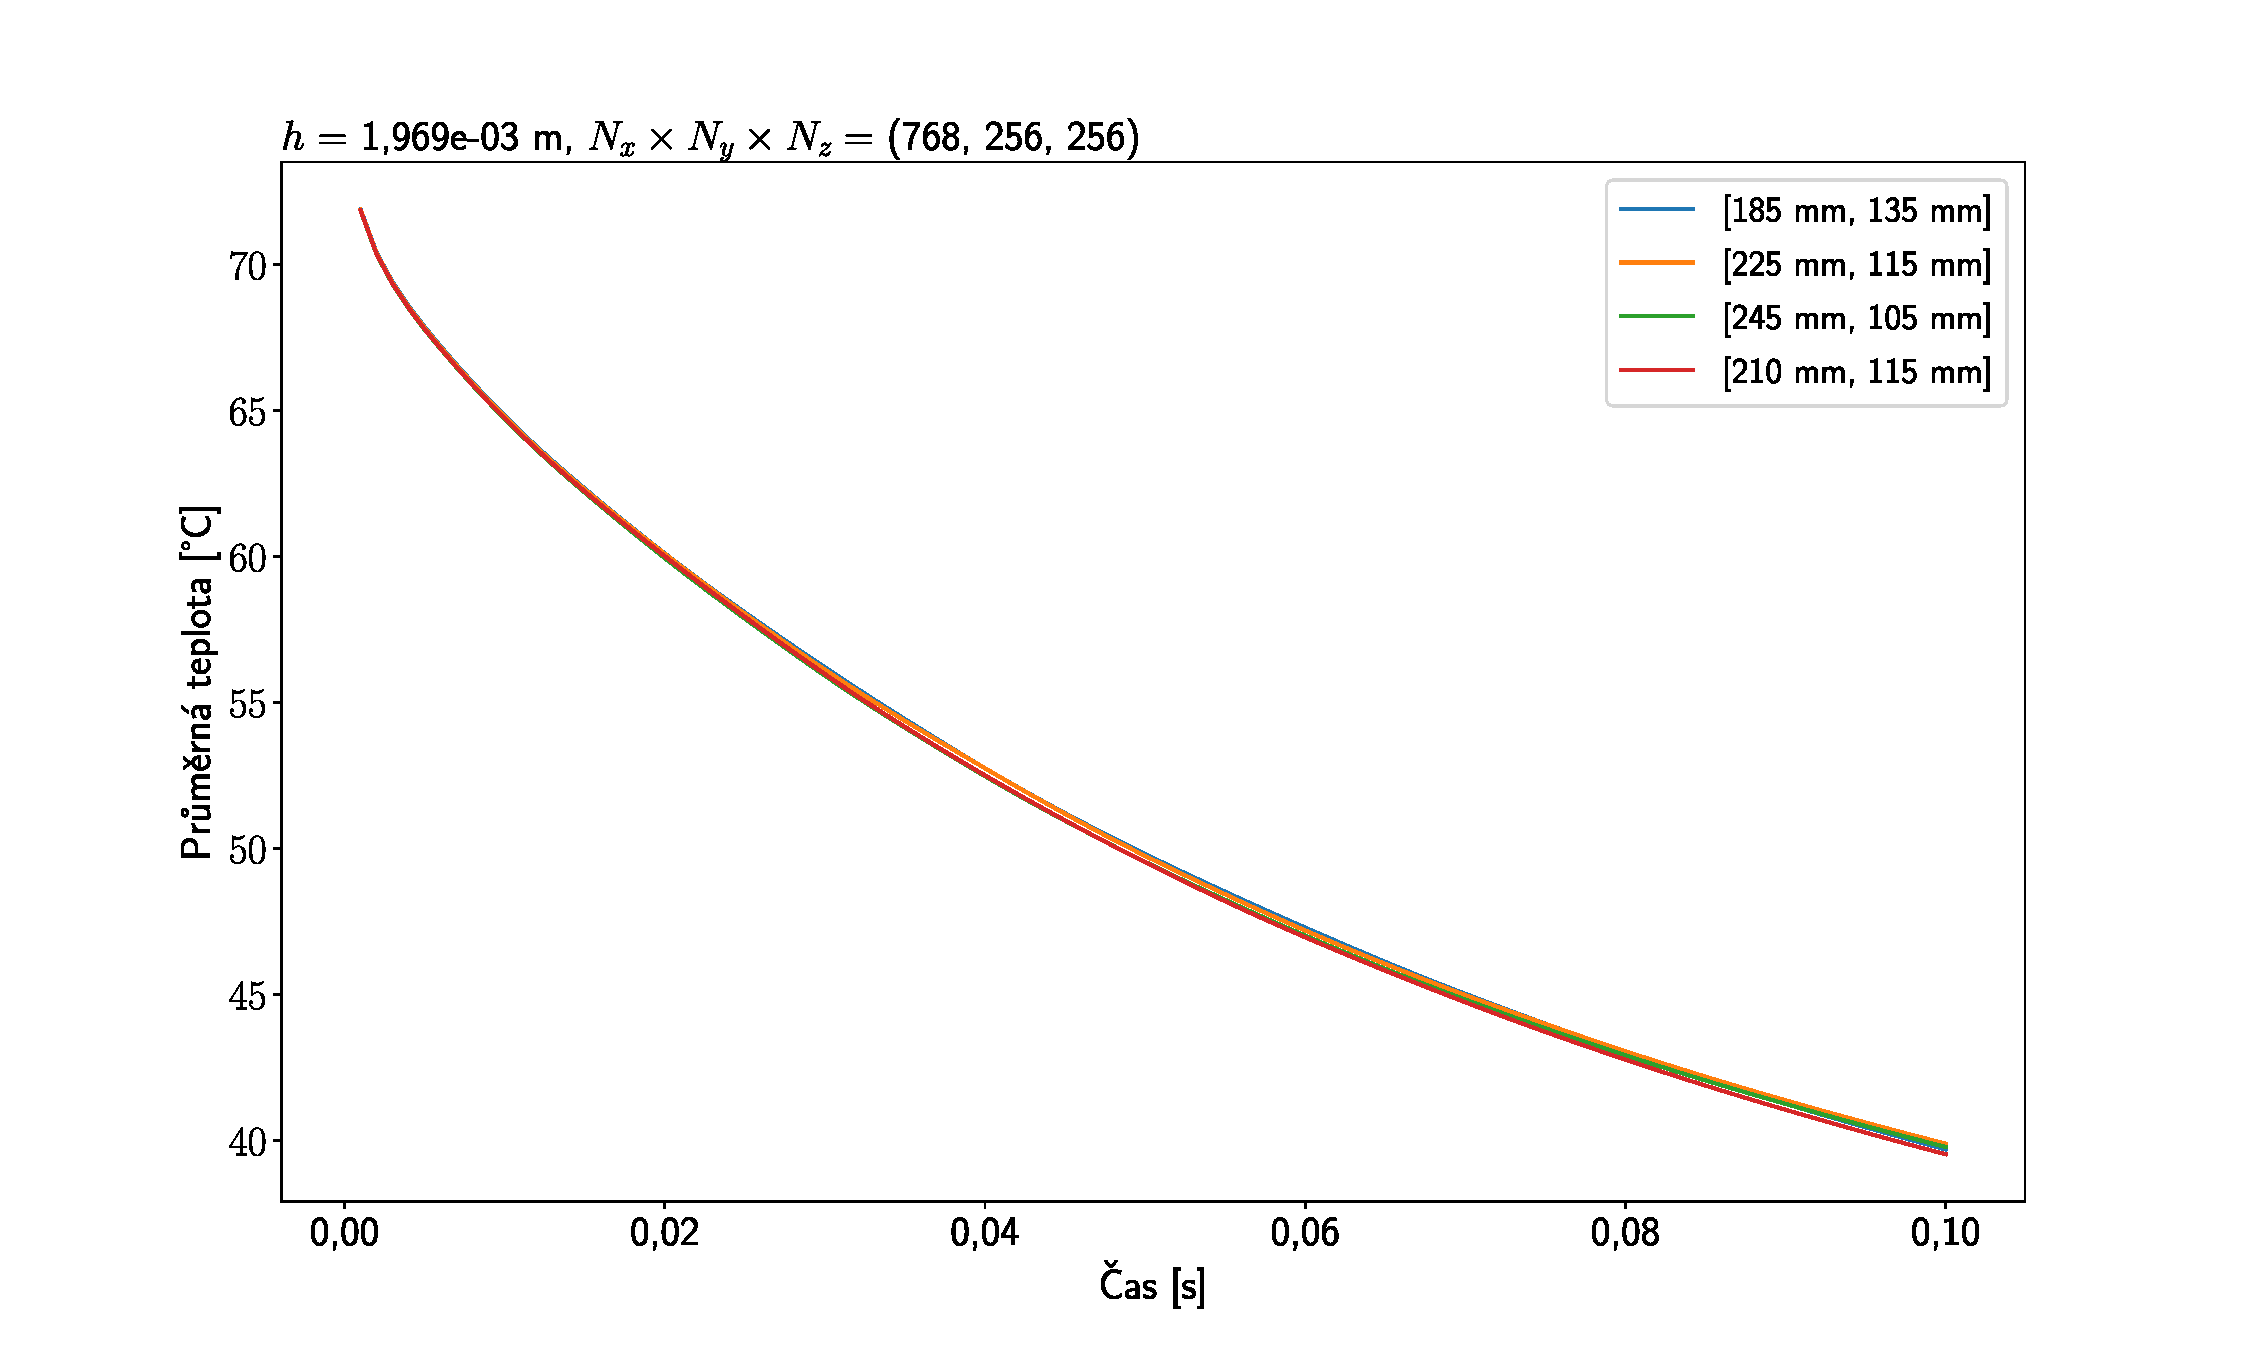
\includegraphics[width=.9\linewidth, clip, trim=3cm 0.65cm 3.5cm 2cm]{Img/Kapitola 3/Probl06_all_rads.pdf}
    %         \end{figure}
    %         \begin{figure}[H]
    %             \centering
    %             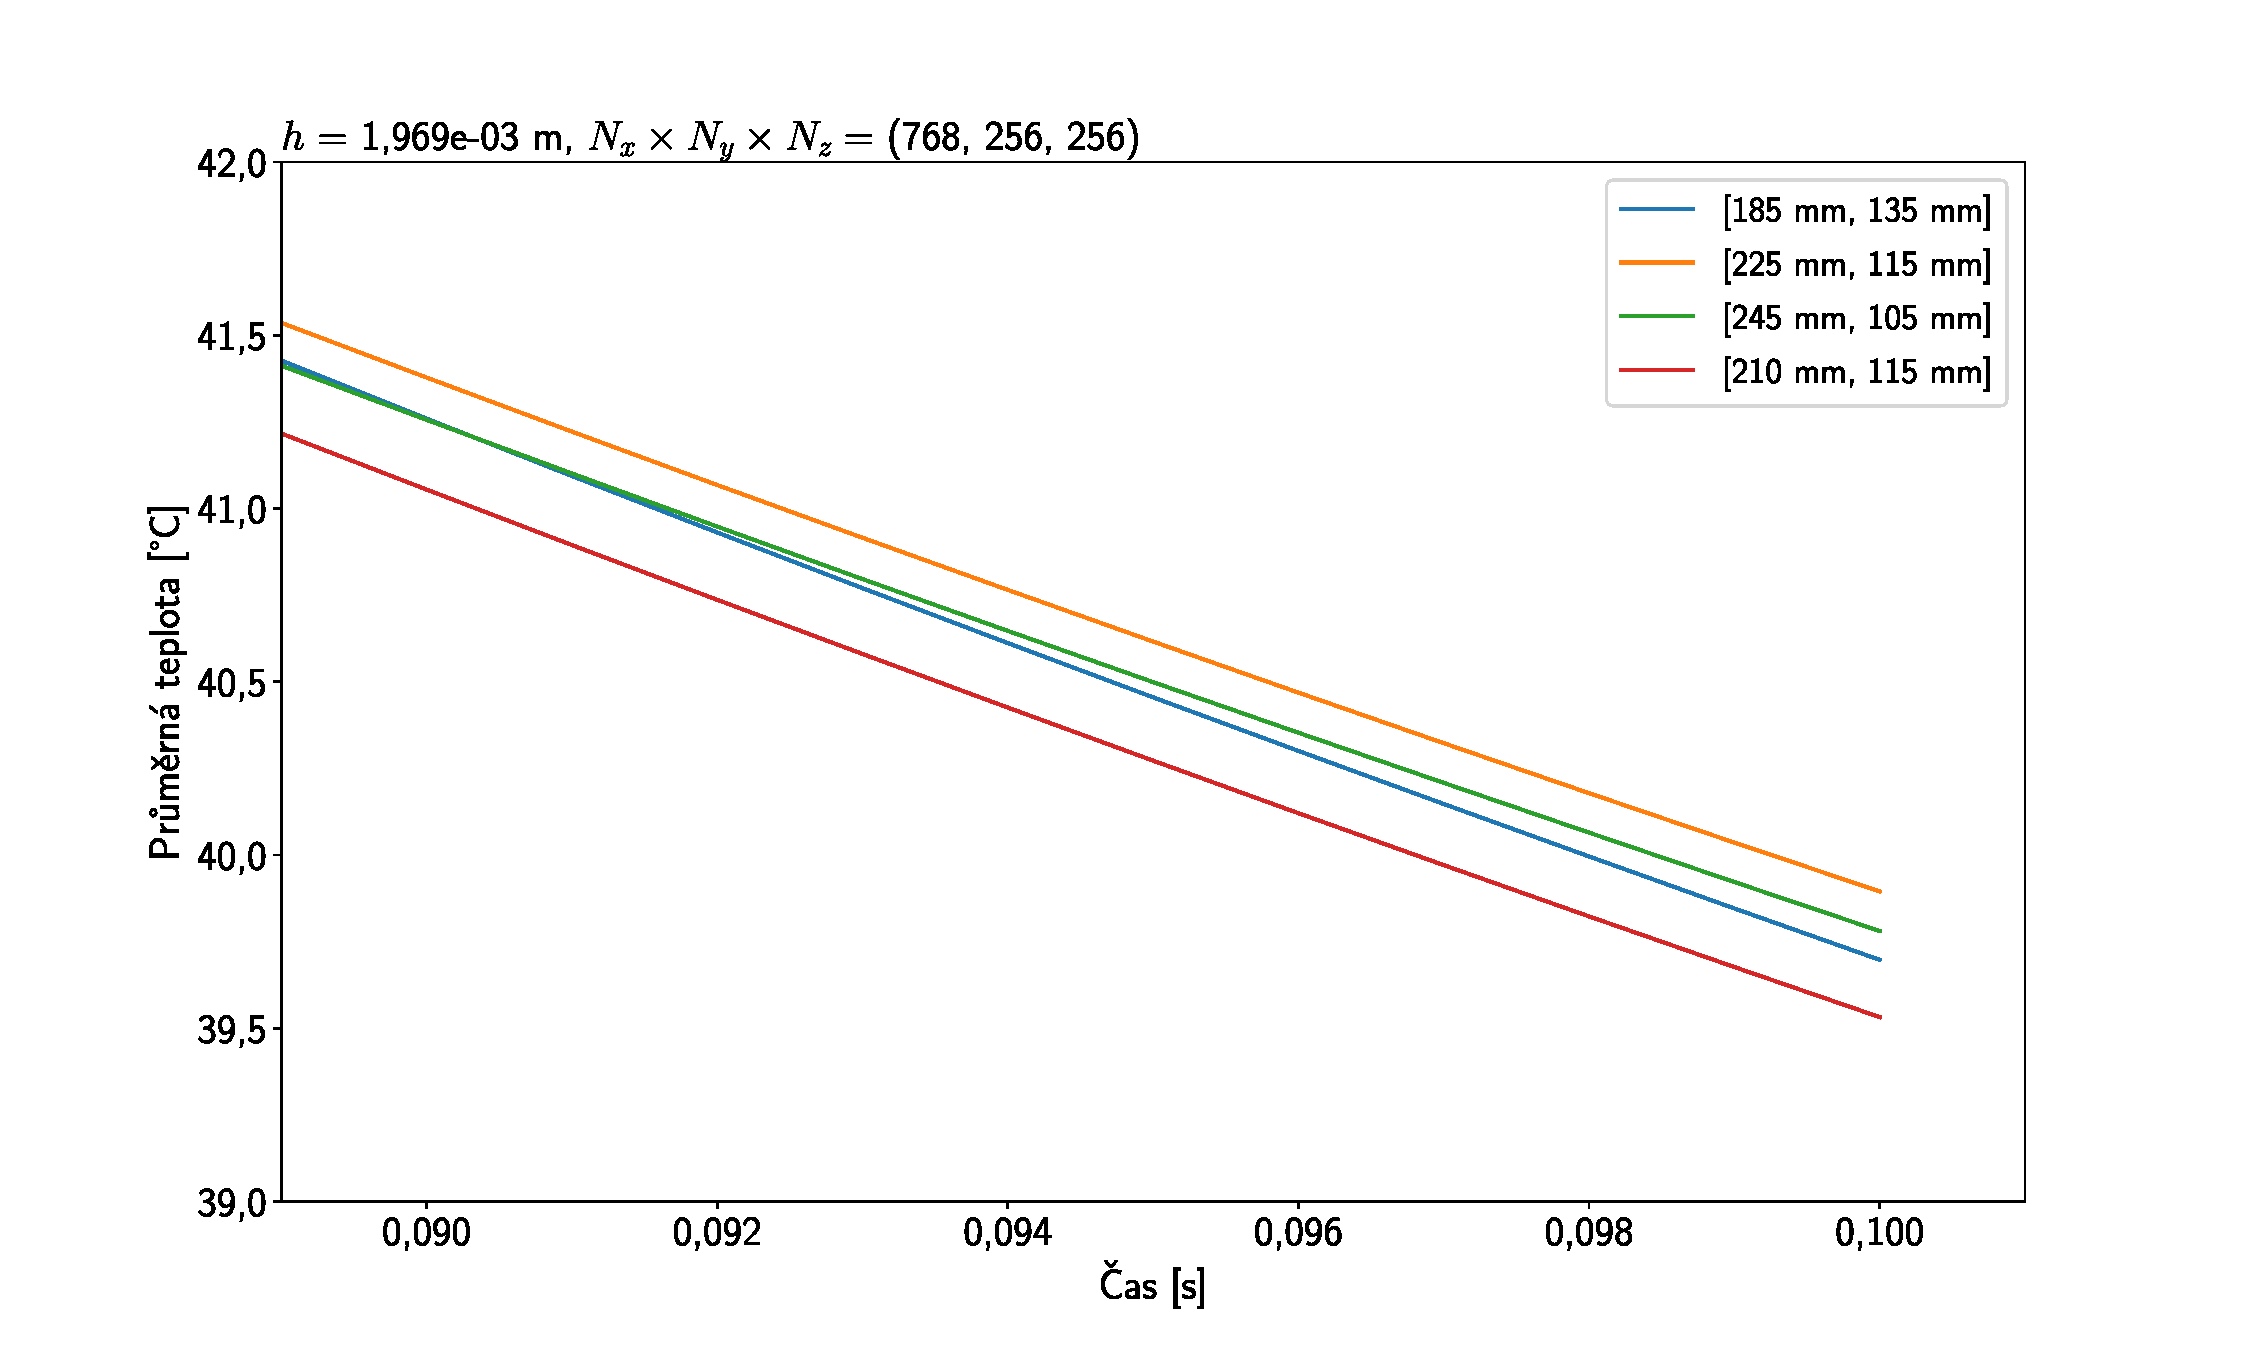
\includegraphics[width=.9\linewidth, clip, trim=2.5cm 0.65cm 3.5cm 2cm]{Img/Kapitola 3/Probl06_all_rads_zoom.pdf}
    %             \caption{Grafy z\'{a}vislosti pr\r{u}m\v{e}rn\'{e} teploty $T_{mean}$ na t\v{e}lese $\Omega_b$ na \v{c}ase $t$ pro \'{u}lohu \ref{sub:Prob06} a pro vybran\'{e} rozm\v{e}ry radi\'{a}toru, prostorov\'{y} krok $h = 1{,}969\cdot 10^{-3} \ \mathrm{m}$ odpov\'{\i}daj\'{\i}c\'{\i} m\v{r}\'{\i}\v{z}ce (768, 256, 256) a \v{c}asov\'{y} krok $\Delta t =  2{,}497 \cdot 10^{-7}$ s. Prvn\'{\i} graf zn\'{a}zor\v{n}uje cel\'{y} \v{c}asov\'{y} pr\r{u}b\v{e}h, ve druh\'{e}m je pro detail p\v{r}ibl\'{\i}\v{z}en fin\'{a}ln\'{\i} \v{c}asov\'{y} \'{u}sek.}
    %             \label{fig:Prob06_rads_all}
    %             \end{figure}

    %     \subsection{V\'{y}sledky \'{u}lohy \ref{sub:Prob06}}

    %         \'{U}loha \ref{sub:Prob06} simuluje nastaven\'{\i} modelu pro r\r{u}zn\'{e} geometrie radi\'{a}toru. P\v{r}edm\v{e}tem zkoum\'{a}n\'{\i} je zde z\'{a}vislost pr\r{u}m\v{e}rn\'{e} teploty radi\'{a}toru $T_{mean}$ na \v{c}ase $t$. Na grafech \ref{fig:Prob06_rads_all} je pro p\v{r}ehlednost vyobrazeno jen n\v{e}kolik r\r{u}zn\'{y}ch velikost\'{\i} radi\'{a}toru. Z graf\r{u} je patrn\'{e}, \v{z}e pro danou \'{u}lohu jsou v\'{y}sledn\'{e} hodnoty pr\r{u}m\v{e}rn\'{e} teploty v intervalu $\langle 39{,}53 ; 39{,}89 \rangle$ \textdegree C. Minim\'{a}ln\'{\i} hodnoty pr\r{u}m\v{e}rn\'{e} teploty je dosa\v{z}eno v p\v{r}\'{\i}pad\v{e} rozm\v{e}r\r{u} chladi\v{c}e $(210,115,25{,}2)$ mm.  

    %     \subsection{Pozn\'{a}mky k hled\'{a}n\'{\i} optim\'{a}ln\'{\i}ho chladi\v{c}e}

    %         V r\'{a}mci t\'{e}to \v{c}\'{a}sti byl hled\'{a}n optim\'{a}ln\'{\i} chladi\v{c}. Model chladi\v{c}e pou\v{z}it\'{y} v t\'{e}to pr\'{a}ci, jak ji\v{z} bylo zm\'{\i}n\v{e}no, neuva\v{z}uje vo\v{s}tinu radi\'{a}toru, a to z d\r{u}vodu vysok\'{y}ch n\'{a}rok\r{u} na rozli\v{s}en\'{\i}. Proto se jedn\'{a} o p\v{r}edb\v{e}\v{z}n\'{y} v\'{y}sledek, kter\'{y} je zat\'{\i}\v{z}en velkou chybou v porovn\'{a}n\'{\i} se skute\v{c}nou situac\'{\i}. B\v{e}hem pokra\v{c}uj\'{\i}c\'{\i}ho v\'{y}zkumu je v pl\'{a}nu zahrnout pokro\v{c}ilej\v{s}\'{\i} geometrii chladi\v{c}e, d\'{\i}ky \v{c}emu\v{z} bude simulace mnohem bl\'{\i}\v{z}e skute\v{c}nosti. 

    \section{Testov\'{a}n\'{\i} konvergence p\v{r}estupov\'{e} okrajov\'{e} podm\'{\i}nky}
        
        V t\'{e}to sekci budeme zkoumat chov\'{a}n\'{\i} teploty v oblasti okolo p\v{r}ek\'{a}\v{z}ky p\v{r}i pou\v{z}it\'{\i} p\v{r}estupov\'{e} okrajov\'{e} podm\'{\i}nky popsan\'{e} v sekci \ref{sec:TraBouCon}. V pr\r{u}b\v{e}hu v\'{y}zkumu byly pozorov\'{a}ny numerick\'{e} chyby v oblasti n\'{a}b\v{e}hov\'{e} hrany p\v{r}ek\'{a}\v{z}ky. 


        Pro optimalizaci v\'{y}po\v{c}tu pou\v{z}ijeme na st\v{e}nu $\Gamma_{top}$ symetrickou okrajovou podm\'{\i}nku, p\v{r}i v\'{y}po\v{c}tech u\v{s}et\v{r}\'{i}me polovinu pam\v{e}ti a budeme tak moci dos\'{a}hnout jemn\v{e}j\v{s}\'{i}ho rozli\v{s}en\'{i} s\'{i}t\v{e}. P\v{r}eci jen p\v{r}ipome\v{n}me, \v{z}e jsme p\v{r}i v\'{y}po\v{c}tech omezen\'{i} pam\v{e}t\'{i} grafick'{y}ch karet, kter\'{a} je st\'{a}le jednou z nejv\v{e}t\v{s}\'{i}ch p\v{r}ek\'{a}\v{z}ek p\v{r}i v\'{y}po\v{c}tu.



        V r\'{a}mci t\'{e}to sekce budeme ve v\'{y}po\v{c}tech sledovat chov\'{a}n\'{i} minim\'{a}ln\'{i} a maxim\'{a}ln\'{i} teploty v podoblasti $\overline{\hat{\Omega_{s}}}$ v\'{y}po\v{c}etn\'{\i} oblasti $\overline{\hat{\Omega}}$. 




   

        
        

        \subsection{P\v{r}estupov\'{a} OP pro $D_* \approx 10^{-3} \ \mathrm{m}^{2} \ \mathrm{s}^{-1}$}
        \label{sub:D10m3}
        
            \begin{tcolorbox}[colframe=blue, title = \'{U}loha \ref{sub:D10m3}]
                        
                Parametry \'{u}lohy:
                \begin{itemize}
                    \begin{multicols}{2}
                    \item $\Omega = (0;1{,}25 \; \mathrm{m}) \times (0;1 \; \mathrm{m}) \times (0;0{,}5 \; \mathrm{m})$,
                    \item $t \in \langle 0;10 \rangle \ \mathrm{s}$,
                    \item $\nu = 1{,}552 \cdot 10^{-5} \ \mathrm{m^2 \ s^{-1}}$,
                    \item $u_{in} = 1 \ \mathrm{m \ s^{-1}}$, 
                    \item $T_{ini,a} = 5 \ ^{\circ}\mathrm{C}$,
                    \item $T_{in} = 5 \ ^{\circ}\mathrm{C}$,
                    \item $T_{ini,b} = 5 \ ^{\circ}\mathrm{C}$,
                    \item $D_{a} = 2{,}239 \cdot 10^{-3} \ \mathrm{m^2 \ s^{-1}}$, 
                    \item $D_b = 9{,}700 \cdot 10^{-3} \ \mathrm{m^2 \ s^{-1}}$,
                    \item $\omega = 0{,}01 \  \mathrm{kg \ s^{-3} \ K^{-1}}$.
                    \end{multicols}
                \end{itemize}
                
                Po\v{c}\'{a}te\v{c}n\'{\i} a okrajov\'{e} podm\'{\i}nky:
                \begin{itemize}
                    \item V $\overline{\hat{\Omega}}$ nastav\'{\i}me po\v{c}\'{a}te\v{c}n\'{\i} podm\'{\i}nky dle sekc\'{\i} \ref{sec:NSEIniCon} a \ref{sec:ADEIniCon}.
                    \item Na \v{c}\'{a}sti hranice $\hat{\Gamma}_{in}$ zvol\'{\i}me vstupn\'{\i} okrajov\'{e} podm\'{\i}nky popsan\'{e} v \ref{sec:NSEIniCon} a \ref{sec:ADEIniCon}.
                    \item Pro $\hat{\Gamma}_{out}$ vol\'{\i}me odtokov\'{e} podm\'{\i}nky dle \ref{sec:NSEIniCon} a \ref{sec:ADEIniCon}.
                    \item Na $\hat{\Gamma}_{w}$ pou\v{z}ijeme bounce-back okrajov\'{e} podm\'{\i}nky ze sekc\'{\i} \ref{sec:NSEIniCon} a \ref{sec:ADEIniCon}.
                    \item Pro t\v{e}leso $\overline{\hat{\Omega}}_b$ vol\'{\i}me n\'{a}sleduj\'{\i}c\'{\i} okrajov\'{e} podm\'{\i}nky: \begin{itemize}
                        \item Pro NSR sch\'{e}ma vol\'{\i}me na $\overline{\hat{\Omega}}_b$ bounce-back okrajovou podm\'{\i}nku dle \ref{sec:NSEIniCon},
                        \item V ADR sch\'{e}matu pou\v{z}ijeme na $\hat{\Gamma}_b$ p\v{r}estupovou podm\'{\i}nku, viz \ref{sec:ADEIniCon}.  
                    \end{itemize}
                \end{itemize}
                
                Parametry LBM:
                \begin{itemize}
                    \item $N_x \times N_y \times N_z \in \{ 40i \times 32i \times 16i\ | \ i \in \{ 3,4,\dots,25 \} \} $,
                    \item $\mathrm{Re} = 33 \ 333$,
                    \item $\nu_{LBM} = 10^{-4}$, odpov\'{\i}d\'{a} $\Delta t \approx 10^{-5} s$.
                \end{itemize}
            \end{tcolorbox}

            \begin{table}[H]
                \centering
                % First subtable
                \begin{tabular}{p{0.25\textwidth}p{0.18\textwidth}p{0.18\textwidth}p{0.18\textwidth}}
                    \toprule
                    \multicolumn{4}{c}{\centering{$t=1.0 \ \mathrm{s}$}} \\ \midrule
                    Rozli\v{s}en\'{\i} s\'{\i}t\v{e} & \multicolumn{1}{p{2.5cm}}{Prostorov\'{y} krok $h \ [\mathrm{m}]$} & \multicolumn{1}{p{2.8cm}}{Minim\'{a}ln\'{\i} teplota $T_{min} \ [^\circ\mathrm{C}]$} & \multicolumn{1}{p{2.8cm}}{Minim\'{a}ln\'{\i} teplota $T_{min} \ [^\circ\mathrm{C}]$} \\ \midrule
                    $160 \times 128 \times 64$  & $7,81 \cdot  10^{-3}$ & 4,757 & 5,587 \\
                    $200 \times 160 \times 80$  & $6,25 \cdot  10^{-3}$ & 4,795 & 5,491 \\
                    $240 \times 192 \times 96$  & $5,21 \cdot  10^{-3}$ & 4,824 & 5,423 \\
                    $280 \times 224 \times 112$  & $4,46 \cdot  10^{-3}$ & 4,845 & 5,367 \\
                    $320 \times 256 \times 128$  & $3,91 \cdot  10^{-3}$ & 4,822 & 5,327 \\
                    $360 \times 288 \times 144$  & $3,47 \cdot  10^{-3}$ & 4,869 & 5,288 \\
                    $400 \times 320 \times 160$  & $3,13 \cdot  10^{-3}$ & 4,864 & 5,258 \\
                    $440 \times 352 \times 176$  & $2,84 \cdot  10^{-3}$ & 4,929 & 5,169 \\ 
                    \bottomrule

                \end{tabular}

                % Single caption for all subtables
                \caption{V\'{y}voj minim\'{a}ln\'{\i} a maxim\'{a}ln\'{\i} teploty v z\'{a}vislosti na rozli\v{s}en\'{\i} s\'{i}t\v{e} pro hodnotu difuzn\'{\i}ho koeficientu $D \approx 10^{-3}$ v \v{c}ase $t = 1 \ \mathrm{s}$.}
                \label{table:D10m3_1}
            \end{table}


            \begin{table}[H]
                \centering
                % First subtable
                \begin{tabular}{p{0.25\textwidth}p{0.18\textwidth}p{0.18\textwidth}p{0.18\textwidth}}
                    \toprule
                    \multicolumn{4}{c}{\centering{$t=3.0 \ \mathrm{s}$}} \\ \midrule
                    Rozli\v{s}en\'{\i} s\'{\i}t\v{e} & \multicolumn{1}{p{2.5cm}}{Prostorov\'{y} krok $h \ [\mathrm{m}]$} & \multicolumn{1}{p{2.8cm}}{Minim\'{a}ln\'{\i} teplota $T_{min} \ [^\circ\mathrm{C}]$} & \multicolumn{1}{p{2.8cm}}{Minim\'{a}ln\'{\i} teplota $T_{min} \ [^\circ\mathrm{C}]$} \\ \midrule
                    $160 \times 128 \times 64$  & $7,81 \cdot  10^{-3}$ & 4,771 & 5,593 \\
                    $200 \times 160 \times 80$  & $6,25 \cdot  10^{-3}$ & 4,802 & 5,494 \\
                    $240 \times 192 \times 96$  & $5,21 \cdot  10^{-3}$ & 4,828 & 5,424 \\
                    $280 \times 224 \times 112$  & $4,46 \cdot  10^{-3}$ & 4,847 & 5,367 \\
                    $320 \times 256 \times 128$  & $3,91 \cdot  10^{-3}$ & 4,865 & 5,322 \\
                    $360 \times 288 \times 144$  & $3,47 \cdot  10^{-3}$ & 4,879 & 5,287 \\
                    $400 \times 320 \times 160$  & $3,13 \cdot  10^{-3}$ & 4,888 & 5,258 \\
                    $440 \times 352 \times 176$  & $2,84 \cdot  10^{-3}$ & 4,931 & 5,169 \\ \bottomrule
                \end{tabular}
                % Single caption for all subtables
                \caption{V\'{y}voj minim\'{a}ln\'{\i} a maxim\'{a}ln\'{\i} teploty v z\'{a}vislosti na rozli\v{s}en\'{\i} s\'{i}t\v{e} pro hodnotu difuzn\'{\i}ho koeficientu $D \approx 10^{-3}$ v \v{c}ase $t = 3 \ \mathrm{s}$.}
                \label{table:D10m3_3}
            \end{table}

            \begin{table}[H]
                \centering
                % First subtable
                \begin{tabular}{p{0.25\textwidth}p{0.18\textwidth}p{0.18\textwidth}p{0.18\textwidth}}
                    \toprule
                    \multicolumn{4}{c}{\centering{$t=5.0 \ \mathrm{s}$}} \\ \midrule
                    Rozli\v{s}en\'{\i} s\'{\i}t\v{e} & \multicolumn{1}{p{2.5cm}}{Prostorov\'{y} krok $h \ [\mathrm{m}]$} & \multicolumn{1}{p{2.8cm}}{Minim\'{a}ln\'{\i} teplota $T_{min} \ [^\circ\mathrm{C}]$} & \multicolumn{1}{p{2.8cm}}{Minim\'{a}ln\'{\i} teplota $T_{min} \ [^\circ\mathrm{C}]$} \\ \midrule
                    $160 \times 128 \times 64$  & $7,81 \cdot  10^{-3}$ & 4,772 & 5,594 \\
                    $200 \times 160 \times 80$  & $6,25 \cdot  10^{-3}$ & 4,803 & 5,497 \\
                    $240 \times 192 \times 96$  & $5,21 \cdot  10^{-3}$ & 4,824 & 5,428 \\
                    $280 \times 224 \times 112$  & $4,46 \cdot  10^{-3}$ & 4,845 & 5,372 \\
                    $320 \times 256 \times 128$  & $3,91 \cdot  10^{-3}$ & 4,864 & 5,324 \\
                    $360 \times 288 \times 144$  & $3,47 \cdot  10^{-3}$ & 4,880 & 5,285 \\
                    $400 \times 320 \times 160$  & $3,13 \cdot  10^{-3}$ & 4,889 & 5,257 \\
                    $440 \times 352 \times 176$  & $2,84 \cdot  10^{-3}$ & 4,930 & 5,172 \\ \bottomrule
                \end{tabular}
                % Single caption for all subtables
                \caption{V\'{y}voj minim\'{a}ln\'{\i} a maxim\'{a}ln\'{\i} teploty v z\'{a}vislosti na rozli\v{s}en\'{\i} s\'{i}t\v{e} pro hodnotu difuzn\'{\i}ho koeficientu $D \approx 10^{-3}$ v \v{c}ase $t = 3 \ \mathrm{s}$.}
                \label{table:D10m3_5}
            \end{table}


            \begin{table}[H]
                \centering
                % First subtable
                \begin{tabular}{p{0.25\textwidth}p{0.18\textwidth}p{0.18\textwidth}p{0.18\textwidth}}
                    \toprule
                    \multicolumn{4}{c}{\centering{$t=10.0 \ \mathrm{s}$}} \\ \midrule
                    Rozli\v{s}en\'{\i} s\'{\i}t\v{e} & \multicolumn{1}{p{2.5cm}}{Prostorov\'{y} krok $h \ [\mathrm{m}]$} & \multicolumn{1}{p{2.8cm}}{Minim\'{a}ln\'{\i} teplota $T_{min} \ [^\circ\mathrm{C}]$} & \multicolumn{1}{p{2.8cm}}{Minim\'{a}ln\'{\i} teplota $T_{min} \ [^\circ\mathrm{C}]$} \\ \midrule
                    $160 \times 128 \times 64$  & $7,81 \cdot  10^{-3}$ & 4,772 & 5,596 \\
                    $200 \times 160 \times 80$  & $6,25 \cdot  10^{-3}$ & 4,802 & 5,497 \\
                    $240 \times 192 \times 96$  & $5,21 \cdot  10^{-3}$ & 4,826 & 5,427 \\
                    $280 \times 224 \times 112$  & $4,46 \cdot  10^{-3}$ & 4,847 & 5,368 \\
                    $320 \times 256 \times 128$  & $3,91 \cdot  10^{-3}$ & 4,863 & 5,325 \\
                    $360 \times 288 \times 144$  & $3,47 \cdot  10^{-3}$ & 4,878 & 5,289 \\
                    $400 \times 320 \times 160$  & $3,13 \cdot  10^{-3}$ & 4,889 & 5,257 \\
                    $440 \times 352 \times 176$  & $2,84 \cdot  10^{-3}$ & 4,932 & 5,168 \\ \bottomrule
                \end{tabular}
                % Single caption for all subtables
                \caption{V\'{y}voj minim\'{a}ln\'{\i} a maxim\'{a}ln\'{\i} teploty v z\'{a}vislosti na rozli\v{s}en\'{\i} s\'{i}t\v{e} pro hodnotu difuzn\'{\i}ho koeficientu $D \approx 10^{-3}$ v \v{c}ase $t = 3 \ \mathrm{s}$.}
                \label{table:D10m3_10}
            \end{table}



            \begin{figure}[h]
                \centering
                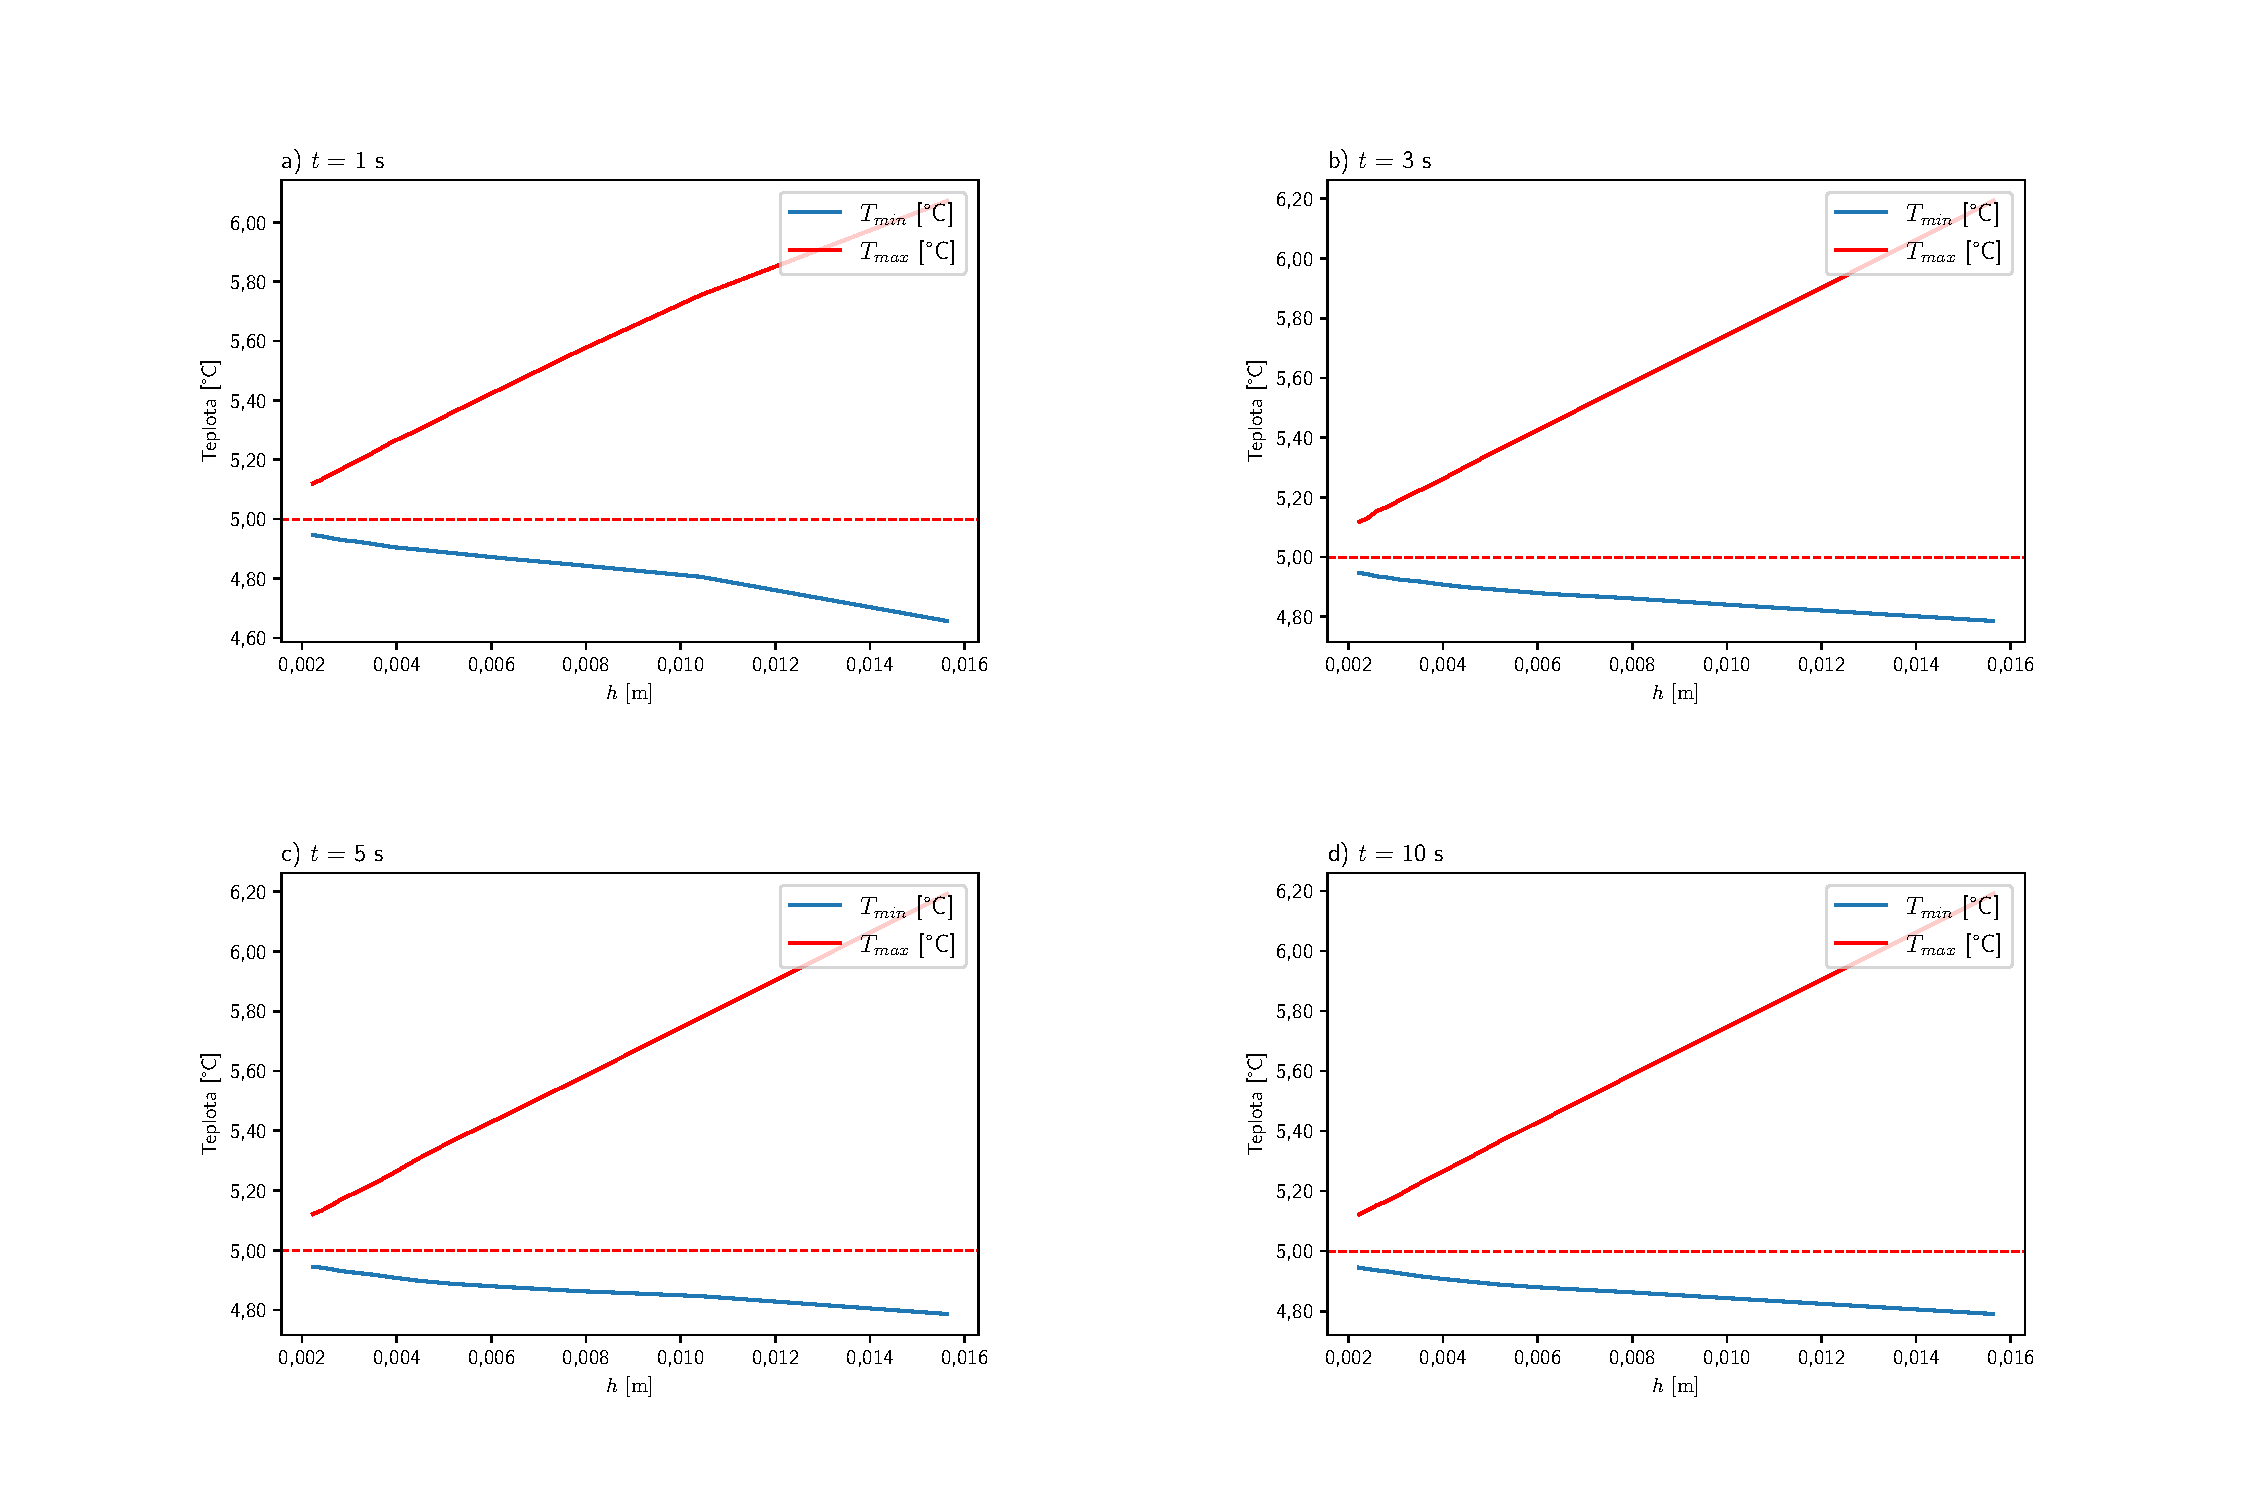
\includegraphics[width=\linewidth, trim=4cm 1cm 4cm 4cm]{Img/Kapitola4/d_10m3.pdf}
                \caption{Grafy zobrazuj\'{\i}c\'{\i} z\'{a}vislost minim\'{a}ln\'{\i} a maxim\'{a}ln\'{\i} teploty na prostorov\'{e}m kroku $h$ pro \'{u}lohu \ref{sub:D10m3} a pro r\r{u}zn\'{e} \v{c}asy $t$.}
                \label{fig:Prob10m3}
            \end{figure}


        \subsection{V\'{y}sledky \'{u}lohy \ref{sub:D10m3}}
    
            \'{U}loha \ref{sub:D10m3} simuluje nastaven\'{\i} p\v{r}estupov\'{e} okrajov\'{e} podm\'{\i}nky v modelu pro r\r{u}zn\'{e} hodnoty prostorov\'{e}ho kroku $h$. P\v{r}edm\v{e}tem zkoum\'{a}n\'{\i} je zde v\'{y}voj minim\'{a}ln\'{i} $T_{min}$ a maxim\'{a}ln\'{i} $T_{max}$ teploty v z\'{a}vislosti zmen\v{s}uj\'{i}c\'{i}m se prostorov\'{e}m kroku $h$. 
            

            % \'{U}loha \ref{sub:Prob02} simuluje nastaven\'{\i} p\v{r}estupov\'{e} okrajov\'{e} podm\'{\i}nky v modelu. P\v{r}edm\v{e}tem zkoum\'{a}n\'{\i} zde je v\'{y}voj pr\r{u}m\v{e}rn\'{e} teploty $T_{mean}$ v \v{c}ase $t$. Na grafu \ref{fig:Prob05_diff_h} pozorujeme z\'{a}vislost pr\r{u}m\v{e}rn\'{e} teploty pro r\r{u}zn\'{e} koeficienty p\v{r}estupu $\omega$ a vstupn\'{\i} rychlost $u_{in} = 1 \ \mathrm{m \ s^{-1}}$. Z grafu je z\v{r}ejm\'{e}, \v{z}e se zvy\v{s}uj\'{\i}c\'{\i} se hodnotou $\omega$ se \'{u}\v{c}innost chlazen\'{\i} zvy\v{s}uje a\v{z} do ur\v{c}it\'{e}ho limitn\'{\i}ho stavu. Na obr\'{a}zku \ref{fig:Probl10_b} je tato situace vyobrazena pro r\r{u}zn\'{e} hodnoty po\v{c}\'{a}te\v{c}n\'{\i} rychlosti $u_{in}$ a pro vybran\'{e} koeficienty p\v{r}estupu $\omega$. Lze nahl\'{e}dnout, \v{z}e i pro vy\v{s}\v{s}\'{\i} hodnoty vstupn\'{\i} rychlosti pr\r{u}m\v{e}rn\'{e} teploty konverguj\'{\i}.
        
            % Z obr\'{a}zku \ref{fig:Probl10_a} lze vy\v{c}\'{\i}st, \v{z}e pro mal\'{e} koeficienty p\v{r}estupu t\'{e}m\v{e}\v{r} nez\'{a}vis\'{\i} na velikosti vstupn\'{\i} rychlosti. Pro hodnoty $\omega$ bl\'{\i}zk\'{e} 1 jsou ji\v{z} rozd\'{\i}ly mezi pr\r{u}m\v{e}rn\'{y}mi teplotami nezanedbateln\'{e}, ale i p\v{r}esto tyto rozd\'{\i}ly nejsou tak markantn\'{\i} v porovn\'{a}n\'{\i} s rychlostmi na vstupu. 









            




        \subsection{P\v{r}estupov\'{a} OP pro $D_* \approx 10^{-5} \ \mathrm{m}^{2} \ \mathrm{s}^{-1}$}
        \label{sub:D10m5}
        
    
            \begin{tcolorbox}[colframe=blue, title = \'{U}loha \ref{sub:D10m5}]
                                    
                Parametry \'{u}lohy:
                \begin{itemize}
                    \begin{multicols}{2}
                    \item $\Omega = (0;1{,}25 \; \mathrm{m}) \times (0;1 \; \mathrm{m}) \times (0;0{,}5 \; \mathrm{m})$,
                    \item $t \in \langle 0;0{,}1 \rangle \ \mathrm{s}$,
                    \item $\nu = 1{,}552 \cdot 10^{-5} \ \mathrm{m^2 \ s^{-1}}$,
                    \item $u_{in} = 1 \ \mathrm{m \ s^{-1}}$, 
                    \item $T_{ini,a} = 5 \ ^{\circ}\mathrm{C}$,
                    \item $T_{in} = 5 \ ^{\circ}\mathrm{C}$,
                    \item $T_{ini,b} = 5 \ ^{\circ}\mathrm{C}$,
                    \item $D_{a} = 2{,}239 \cdot 10^{-3} \ \mathrm{m^2 \ s^{-1}}$, 
                    \item $D_b = 9{,}700 \cdot 10^{-3} \ \mathrm{m^2 \ s^{-1}}$,
                    \item $\omega = 0{,}01 \  \mathrm{kg \ s^{-3} \ K^{-1}}$.
                    \end{multicols}
                \end{itemize}
                
                Po\v{c}\'{a}te\v{c}n\'{\i} a okrajov\'{e} podm\'{\i}nky:
                \begin{itemize}
                    \item V $\overline{\hat{\Omega}}$ nastav\'{\i}me po\v{c}\'{a}te\v{c}n\'{\i} podm\'{\i}nky dle sekc\'{\i} \ref{sec:NSEIniCon} a \ref{sec:ADEIniCon}.
                    \item Na \v{c}\'{a}sti hranice $\hat{\Gamma}_{in}$ zvol\'{\i}me vstupn\'{\i} okrajov\'{e} podm\'{\i}nky popsan\'{e} v \ref{sec:NSEIniCon} a \ref{sec:ADEIniCon}.
                    \item Pro $\hat{\Gamma}_{out}$ vol\'{\i}me odtokov\'{e} podm\'{\i}nky dle \ref{sec:NSEIniCon} a \ref{sec:ADEIniCon}.
                    \item Na $\hat{\Gamma}_{w}$ pou\v{z}ijeme bounce-back okrajov\'{e} podm\'{\i}nky ze sekc\'{\i} \ref{sec:NSEIniCon} a \ref{sec:ADEIniCon}.
                    \item Pro t\v{e}leso $\overline{\hat{\Omega}}_b$ vol\'{\i}me n\'{a}sleduj\'{\i}c\'{\i} okrajov\'{e} podm\'{\i}nky: \begin{itemize}
                        \item Pro NSR sch\'{e}ma vol\'{\i}me na $\overline{\hat{\Omega}}_b$ bounce-back okrajovou podm\'{\i}nku dle \ref{sec:NSEIniCon},
                        \item V ADR sch\'{e}matu pou\v{z}ijeme na $\hat{\Gamma}_b$ p\v{r}estupovou podm\'{\i}nku, viz \ref{sec:ADEIniCon}.  
                    \end{itemize}
                \end{itemize}
                
                Parametry LBM:
                \begin{itemize}
                    \item $N_x \times N_y \times N_z \in \{ 40i \times 32i \times 16i\ | \ i \in \{ 3,4,\dots,25 \} \} $,
                    \item $\mathrm{Re} = 33 \ 333$,
                    \item $\nu_{LBM} = 10^{-4}$, odpov\'{\i}d\'{a} $\Delta t \approx 10^{-5} s$.
                \end{itemize}

            \end{tcolorbox}

    \section{Experiment CUBI}

        V t\'{e}to sekci se zam\v{e}\v{r}\'{i}me na simulaci prob\'{i}haj\'{i}c\'{i}ho experimentu ve v\'{y}zkumn\'{e}m centru SENSE, v americk\'{e}m ...
        
        Projekt zkoum\'{a} v\'{y}voj rychlostn\'{i}ho a teplotn\'{i}ho profilu v oblasti mezn\'{i} vrstv\v{e} okolo p\v{r}ek\'{a}\v{z}ky - tzv. CUBIho. Experiment prob\'{i}h\'{a} ve v\v{e}trn\'{e}m tunelu, jeho\v{z} pr\r{u}\v{r}ez je ve tvaru \v{c}terve o hran\v{e} $1 \ \mathrm{m}$.
        
        Uva\v{z}ujme tedy v\'{y}po\v{c}etn\'{\i} oblast $\overline{\hat{\Omega}}$. P\v{r}ek\'{a}\v{z}ku $\overline{\hat{\Omega}}_b$ v tomto p\v{r}\'{\i}pad\v{e} bude tvo\v{r}it t\v{e}leso slo\v{z}en\'{e} ze t\v{r}\'{\i} toto\v{z}n\'{y}ch krychl\'{\i} o hran\v{e} $0.125 \ \mathrm{m}$ sestaven\'{y}ch do tvaru p\'{i}smene L, viz. obr\'{a}zek \ref{fig:CUBI}. Toto t\v{e}leso dostalo jm\'{e}no CUBI.

        \begin{figure}[H]
            \centering
            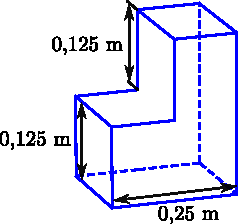
\includegraphics{Img/Kapitola4/CUBI.pdf}
            \caption{Sch\'{e}ma CUBIho s vyzna\v{c}en\'{y}mi rozm\v{e}ry.}
            \label{fig:CUBI}
        \end{figure}

        P\v{r}i implementaci tohoto experimentu byla pou\v{z}ita symerick\'{a} okrajov\'{a} podm\'{\i}nka \ref{sec:SymBouCon}. To bylo mo\v{z}n\'{e} prov\'{e}st z podstaty \'{u}lohy. Jeliko\v{z} je v\'{y}\v{s}ka p\v{r}ek\'{a}\v{z}ky v porovn\'{a}n\'{i} s v\'{y}\v{s}kou tunelu mal\'{a}, proud\v{e}n\'{\i} ve vrchn\'{i} polovin\v{e} tunelu se st\'{a}v\'{a} lamin\'{a}rn\'{i}m a tud\'{i}\v{z} pro n\'{a}s nezaj\'{i}mav\'{y}m.

        Velkou v\'{y}hodou pou\v{z}it\'{i} t\'{e}to okrajov\'{e} podm\'{i}nky je u\v{s}et\v{r}en\'{i} poloviny pam\v{e}ti, co\v{z} n\'{a}m umo\v{z}n\'{i} dohs\'{a}hnout jemn\v{e}j\v{s}\'{i}ho rozli\v{s}en\'{i}. 


        P\v{r}edm\v{e}tem z\'{a}jmu pro n\'{a}s bude rychlostn\'{i} a teplotn\'{i} profil t\v{e}sn\v{e} nad povrchem spodn\'{i} st\v{e}ny v\'{y}po\v{c}etn\'{i} oblasti $\overline{\hat{\Omega}}$. Nastaven\'{i} v\'{y}po\v{c}etn\'{i} oblasti pro simulace bude jako na obr\'{a}zku \ref{fig:ProblCUBI_domain}.


        \begin{figure}[H]
            \centering
            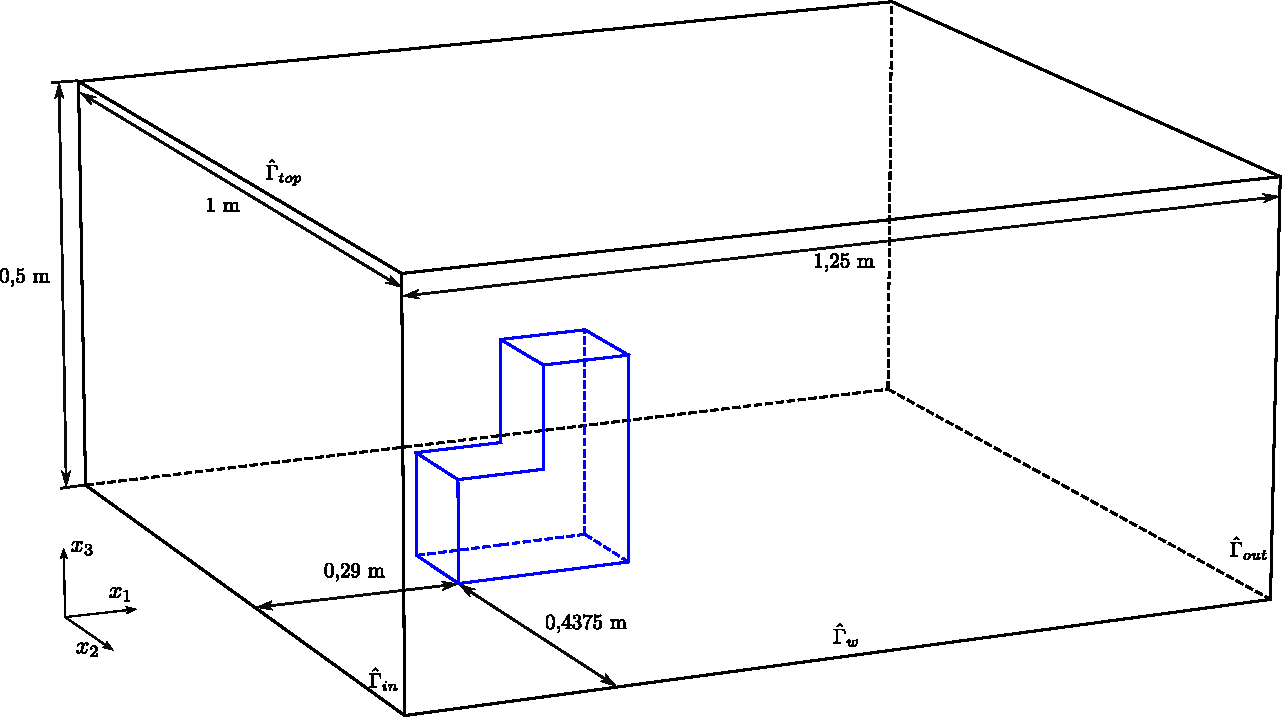
\includegraphics[width=\textwidth]{Img/Kapitola4/CUBI_domain.pdf}
            \caption{Sch\'{e}ma v\'{y}po\v{c}etn\'{i} oblasti pro \'{u}lohu \ref{sub:ProbCUBI}.}
            \label{fig:CUBI_domain}
        \end{figure}

        \subsection{Experiment CUBI}
        \label{sub:ProbCUBI}

            \begin{tcolorbox}[colframe=blue, title = \'{U}loha \ref{sub:ProbCUBI}]
                                        
                Parametry \'{u}lohy:
                \begin{itemize}
                    \begin{multicols}{2}
                    \item $\Omega = (0;1{,}25 \; \mathrm{m}) \times (0;1 \; \mathrm{m}) \times (0;0{,}5 \; \mathrm{m})$,
                    \item $t \in \langle 0;0{,}1 \rangle \ \mathrm{s}$,
                    \item $\nu = 1{,}552 \cdot 10^{-5} \ \mathrm{m^2 \ s^{-1}}$,
                    \item $u_{in} = 1 \ \mathrm{m \ s^{-1}}$, 
                    \item $T_{ini,a} = 5 \ ^{\circ}\mathrm{C}$,
                    \item $T_{in} = 5 \ ^{\circ}\mathrm{C}$,
                    \item $T_{ini,b} = 5 \ ^{\circ}\mathrm{C}$,
                    \item $D_{a} = 2{,}239 \cdot 10^{-3} \ \mathrm{m^2 \ s^{-1}}$, 
                    \item $D_b = 9{,}700 \cdot 10^{-3} \ \mathrm{m^2 \ s^{-1}}$,
                    \item $\omega = 0{,}01 \  \mathrm{kg \ s^{-3} \ K^{-1}}$.
                    \end{multicols}
                \end{itemize}
                
                Po\v{c}\'{a}te\v{c}n\'{\i} a okrajov\'{e} podm\'{\i}nky:
                \begin{itemize}
                    \item V $\overline{\hat{\Omega}}$ nastav\'{\i}me po\v{c}\'{a}te\v{c}n\'{\i} podm\'{\i}nky dle sekc\'{\i} \ref{sec:NSEIniCon} a \ref{sec:ADEIniCon}.
                    \item Na \v{c}\'{a}sti hranice $\hat{\Gamma}_{in}$ zvol\'{\i}me vstupn\'{\i} okrajov\'{e} podm\'{\i}nky popsan\'{e} v \ref{sec:NSEIniCon} a \ref{sec:ADEIniCon}.
                    \item Pro $\hat{\Gamma}_{out}$ vol\'{\i}me odtokov\'{e} podm\'{\i}nky dle \ref{sec:NSEIniCon} a \ref{sec:ADEIniCon}.
                    \item Na $\hat{\Gamma}_{w}$ pou\v{z}ijeme bounce-back okrajov\'{e} podm\'{\i}nky ze sekc\'{\i} \ref{sec:NSEIniCon} a \ref{sec:ADEIniCon}.
                    \item Na vrchn\'{i} st\v{e}nu $\hat{\Gamma}_{top}$ p\v{r}edep\'{i}\v{s}eme symetrickou okrajovou podm\'{i}nku \ref{sec:SymBouCon}. 
                    \item Pro t\v{e}leso $\overline{\hat{\Omega}}_b$ vol\'{\i}me n\'{a}sleduj\'{\i}c\'{\i} okrajov\'{e} podm\'{\i}nky: \begin{itemize}
                        \item Pro NSR sch\'{e}ma vol\'{\i}me na $\overline{\hat{\Omega}}_b$ bounce-back okrajovou podm\'{\i}nku dle \ref{sec:NSEIniCon},
                        \item V ADR sch\'{e}matu pou\v{z}ijeme na $\hat{\Gamma}_b$ p\v{r}estupovou podm\'{\i}nku, viz \ref{sec:ADEIniCon}.  
                    \end{itemize}
                \end{itemize}
                
                Parametry LBM:
                \begin{itemize}
                    \item $N_x \times N_y \times N_z \in \{ 40i \times 32i \times 16i\ | \ i \in \{ 3,4,\dots,25 \} \} $,
                    \item $\mathrm{Re} = 33 \ 333$,
                    \item $\nu_{LBM} = 10^{-4}$, odpov\'{\i}d\'{a} $\Delta t \approx 10^{-5} s$.
                \end{itemize}
            \end{tcolorbox}

        \subsection{V\'{y}sledky \'{u}lohy \ref{sub:ProbCUBI}}
        

        

